\documentclass[11pt, dvipdfmx]{jarticle}

\usepackage[dvipdfmx]{graphicx}
\usepackage{sty/fancyheadings}
\usepackage{sty/sotsuron2009}
\usepackage{here}
\usepackage{ascmac}
\usepackage[subrefformat=parens]{subcaption}
\usepackage{here}
\usepackage{cite}
\usepackage{amsmath}
\pagestyle{empty}
\usepackage{bm}
\usepackage{comment}
\usepackage{setspace}
\usepackage{autobreak}
\usepackage{pdfpages}
\linesparpage{40}
%\makeatletter
%\renewcommand{\theequation}{
%\thesection.\arabic{equation}}
%\@addtoreset{equation}{section}
%\makeatother
\pagestyle{fancy}

\newcommand{\argmin}{\mathop{\rm arg~min}\limits}
\newcommand{\Section}[1]{\section*{#1}
\addcontentsline{toc}{section}{#1}}
\newcommand{\Subsection}[1]{\section*{#1}
\addcontentsline{toc}{subsection}{#1}}
\renewcommand{\refname}{}


\begin{document}
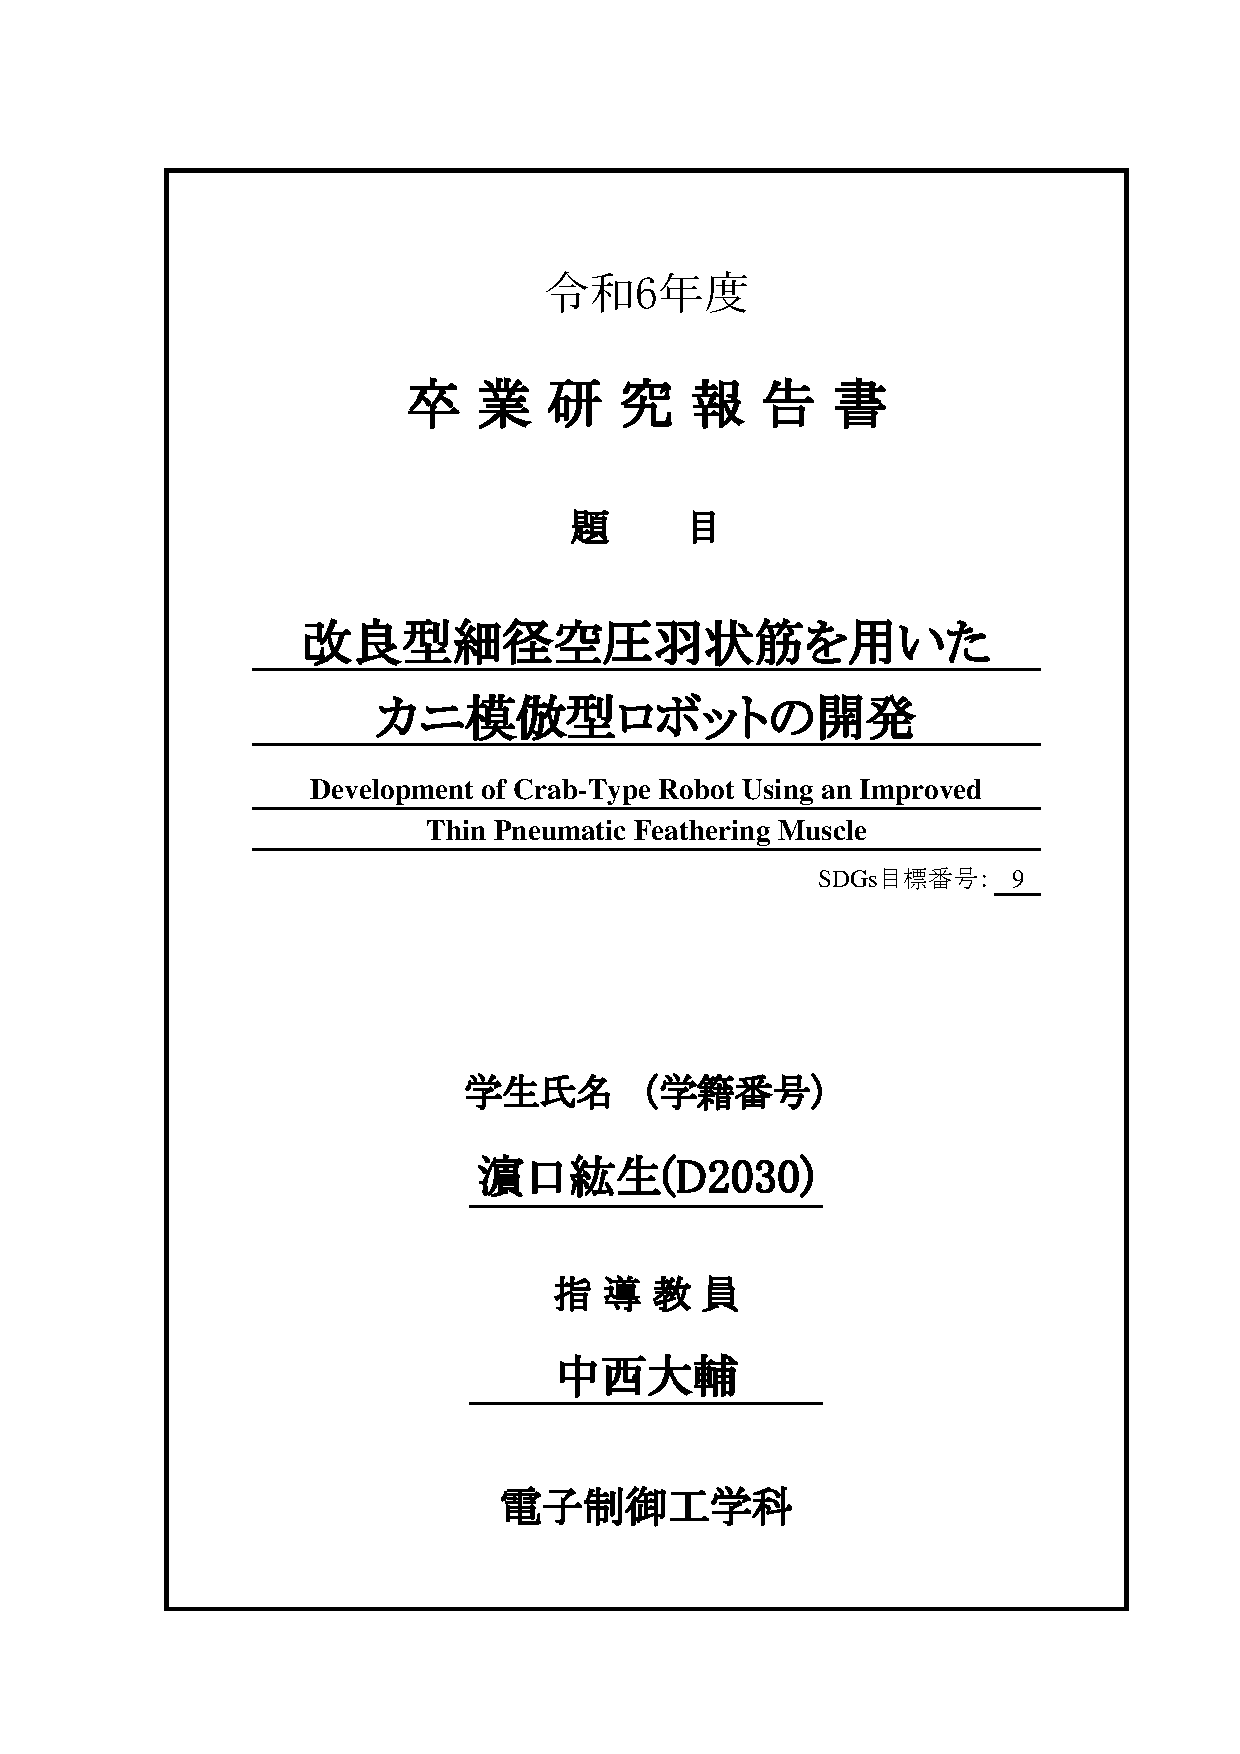
\includepdf[pages=-]{hyoushi.pdf}

\thispagestyle{empty}
\newpage
\section*{概要}
McKibben型空気圧人工筋(McKibben Pneumatic Actuator,以下MPA)は圧縮空気を入力することで収縮し,自身の軸方向への張力を発生させるアクチュエータであり,近年では直径数mmの細径MPAが注目されている.
細径MPAは生体筋に似た特性を持ち,筋骨格系ロボットや生物模倣ロボットに用いられてきた.
一方,甲殻類や昆虫を模した外骨格を有する生物模倣ロボットでは,外骨格内部へのアクチュエータの配置が困難なため,主にワイヤ駆動やサーボモータを使用したものが主流であったが,実際の生物の構成と相違点が出てきてしまう問題点があった.
これに対して先行研究では細径MPAを用いた羽状筋の開発が行われた.またズワイガニを実際に解剖して得られた計測データを参考にし歩脚ロボットを開発し,細径空圧羽状筋によって関節を開閉動作させることに成功した.
一方で,細径MPAの制作方法や羽状筋の構成,および関節構造の再現など様々な点で課題が残された.
本研究ではこれらの先行研究の課題点を改良した細径空圧羽状筋とロボットの開発を行った.
長節から指節までの節の開閉動作を実機によって確認し,全ての関節について概ね設計通りの可動域が実現できていることを確認した.
特に長節-腕節間関節については,実際のカニと同等の可動域が再現できていることを確認した.
今後は腱の固定方法と可動域の計算の際に用いた数理モデルの改良を行い,実際のカニの可動域に近い動きをする歩脚ロボットの開発を目指す.
\newpage
\section*{Abstract}
The McKibben Pneumatic Actuator (MPA) is an actuator that contracts when compressed air is applied to it, generating tension in its own axial direction.
Recently, thin MPAs with a diameter of a few millimeters have been attracting attention.
On the other hand, biomimetic robots with exoskeletons that mimic crustaceans and insects have mainly used wire drives and servo motors due to the difficulty of placing actuators inside the exoskeleton, but there are some differences from actual biological structures.
In response to this problem, previous research developed a feather-shaped muscle using a thin MPA. In addition, a gait robot was developed based on measurement data obtained by dissecting a snow crab, and the joints were successfully opened and closed using thin pneumatic pterostome muscles.
On the other hand, there are still various issues to be solved, such as the production method of the thin MPA, the composition of the pterygoid muscles, and the reproduction of the joint structure.
In this study, we developed a robot with a thin pneumatic winged muscle that improves on these issues in previous studies.
We confirmed that all joints were able to achieve the designed range of motion.
In particular, we confirmed that the range of motion of the joint between the long segment and the brachial segment was equivalent to that of an actual crab.
In the future, we will improve the method of tendon fixation and the mathematical model used to calculate the range of motion, and aim to develop a walking leg robot that can move in a range of motion similar to that of an actual crab.        % 概要
\thispagestyle{empty}
\newpage
\tableofcontents
\thispagestyle{empty}

%章ごとに呼び出し

\newpage
\setcounter{page}{1}
\section{緒言}
McKibben型空気圧人工筋(McKibben Pneumatic Actuator,以下MPA)は圧縮空気を入力することで収縮し,自身の軸方向への張力を発生させるアクチュエータである\cite{2003722}.
従来は直径が数十mm程度のMPAを用いたロボットに関する応用研究が盛んに行われてきたが,近年では直径が数mm程度の細径MPAが注目を集めている\cite{wakimoto}.
細径MPAは従来のものより細くしなやかであり生体筋に似た特徴から小さな筋肉,あるいは集積によって単純な紡錘型以外の筋肉を表現可能なため,筋骨格系ロボットや生物模倣ロボットなどに盛んに用いられてきた\cite{森田隆介2016}\cite{森和也2014}.

一方で甲殻類や昆虫などを模した外骨格生物模倣ロボットに関しては外骨格内部へアクチュエータを配置することが困難なことから,関節にサーボモータを配置したもの\cite{jmse10121804}が主流となっている.
このようなロボットは外骨格生物の外形こそ再現できているものの,実際の生物の構成や駆動原理からして異なる.
また「構成要素が外骨格内にすべて納まっている」という外骨格ならではのメリットも,実現できているとは言い難い.
これに対して前述の細径MPAは,その細さやしなやかさから細長い外骨格内部に配置可能であり,また集積することで実際の生物のような羽状筋も表現することが可能である\cite{2003}.

そこで本研究では細径MPAを用いた外骨格生物模倣ロボットの開発を行う.
先行研究\cite{hasegawa}では外骨格生物のなかでも甲殻類の蟹(ズワイガニ)をモデル生物として設定し,これの歩脚を模倣したロボットの開発に向けて,細径MPAおよびそれを用いた羽状筋の開発が行われた.
またズワイガニを実際に解剖して得られた計測データを参考生歩脚ロボットを開発し,細径空圧羽状筋によって関節を開閉動作させることに成功した\cite{hasegawa}.
一方で,先行研究\cite{hasegawa}で開発された細径空圧羽状筋およびロボットにはいくつかの問題が確認された.
まず,先行研究で用いられた細径MPA作製方法は煩雑であり,作製に時間と練度が必要であった.また収縮性能が低いことや,羽状筋の細径MPAの根元の角度が固定されており,
収縮時に羽状角が変化できずに腱の引き込みを妨げていた.またロボットの関節部についても腱の付着構造に問題があり,可動域の再現などはできていなかった.

そこで本研究では,改めてカニの解剖を行い,関節構造などを確認した.さらに前述した課題点を見直した改良細径空圧筋およびロボットを開発した.
本論文の構成は以下の通りである.まず2章では,本研究で用いる細径MPAに関する特徴と先行研究について述べてから,本研究で開発に成功した細径MPAの作製方法を紹介する.
次に3章では,本研究でモデル生物として扱う蟹の構成と筋構造について実際にズワイガニを解剖して得た知見などを基に述べる.
最後に4章では模倣ロボットを作製するにあたって集積細径MPAを用いた羽状筋の開発について述べたのち,ズワイガニをモデルにした歩脚ロボットの開発とその動作実験について述べる.

% 代表的な人工筋肉として,圧縮空気により骨格筋のように収縮するMcKibben 型空気圧人工筋肉(MPA) があげられる.
% 従来は直径が数十mm 程度のものが多かったが,近年では数mm 程度の細径のMPA が注目を集めている\cite{wakimoto}.
% その細さを生かして小さな筋肉,あるいは集積によって単純な紡錘型以外の筋肉を表現可能なことから,筋骨格系ロボットにおいて特に盛んに用いられている\cite{wakimoto}.
% 一方で甲殻類をはじめとする外骨格系ロボットについては,ワイヤ駆動や関節にサーボモータを配置したものが主流であった\cite{jmse10121804}.
% これは骨格内部にアクチュエータを配置することが困難だからである.
% 細径MPA であれば骨格内部にアクチュエータを配置することが可能であり,実際の生物に近い構成でロボットを作製することが可能である.
% そこで本研究では外骨格生物のうち甲殻類の蟹をモデルに,実際の蟹の筋構造を参考にして細径MPA を使用した蟹の歩脚ロボットの開発に取り組む.
    % 緒言
%\newpage
\section{先行研究の内容}
%%%%%%%%%%%%%%%%%%%%%%%%%%%%%%%%%%%%%%%%%%%%%%%%%%%%%%%%%
\subsection{McKibben型空気圧人工筋肉アクチュエータ(MPA)}
% ・今のとこは先輩のやつを真似ただけ.
MPAはシリコンゴムチューブをナイロンメッシュで覆うことで構成されており(図\ref{fig:MPA}\subref{fig:Structure}),両端に栓をするシンプルな構造である.
これに圧縮した空気を印加することでシリコンゴムチューブが膨張しメッシュによる自身の軸方向への張力が発生するアクチュエータである(図\ref{fig:MPA}\subref{fig:move}).
高出力かつ素材自体も軽量で,物理的柔軟性による高い弾性力を持つという利点があり,筋肉の代用として生物を模したロボットやリハビリなどに用いられる\cite{2003722}.
%%%%%%%%%%%%%%%%%%%%%%%%%%%%%%%%%%%%%%%%%%%%%%%%%%%%%%%%%
\begin{figure}[b]
  %
  \begin{minipage}{0.49\columnwidth}
    \vspace{4mm}
    \centering
    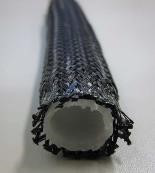
\includegraphics[scale=1]{image/MPA_kousei.png}
    \vspace{3mm}
    \subcaption{MPA断面図}
    \label{fig:Structure}
  \end{minipage}
  %
  \begin{minipage}{0.49\columnwidth}
    \vspace{10mm}
    \centering
    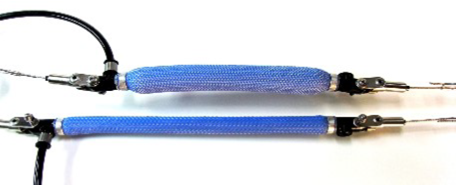
\includegraphics[scale=.8]{image/MPA_dousa.png}
    \vspace{10mm}
    \subcaption{MPA外観および動作の様子}
    \label{fig:move}
  \end{minipage}
  %
  \caption{McKibben型空気圧人工筋(MPA)の構成および外観\cite{中西大輔2020}}
  \label{fig:MPA}
\end{figure}
%%%%%%%%%%%%%%%%%%%%%%%%%%%%%%%%%%%%%%%%%%%%%%%%%%%%%%%%%
\subsection{細径MPA}
% ・脇本修一の論文を参考に細径MPAの冗長性,従来のMPAとの比較などについて説明,φ3のMPAの写真
従来のMPAは外径が十数mm程のものであったのに対し,細径MPAは外径が数mm程のものである.
先行研究\cite{hasegawa}で用いられた細径MPAについて説明する.図\ref{fig:campare}には,先行研究\cite{hasegawa}で開発した外径5 mmおよび3 mmの細径MPAと,外径12 mmの従来のMPAを示す.
細径化には下記のような利点があると考えられている\cite{wakimoto}\cite{1390282680917523328}.
\begin{enumerate}
  \item 非常にしなやかな人工筋となり座屈することなく任意形状での配置や集積が可能
  \item 集積化により収縮量を増大させることが可能
  \item 集積化により冗長性を持ちシステムの安全性が向上
\end{enumerate}
MPAの収縮力は断面積に比例するため,細径MPAは従来のものに比べると発生する張力は小さいものの,細くしなやかであり任意形状での配置や集積化が可能である.
生体筋と柔らかさや動作が似ていることから,紡錘状に集積し筋骨格系ロボット(図\ref{fig:saikei}\subref{fig:kin})へ応用したり,生物模倣ロボットとしてタコ腕模倣メカニズム(図\ref{fig:saikei}\subref{fig:tako})も開発されており,曲げ動作やねじり動作を実現している\cite{森和也2014}.
%%%%画像置き場%%%%%%%%%%%%%%%%%%%%%%%%%%%%%%%%%%%%%%%%%%%%
\begin{figure}[t]
  \centering
  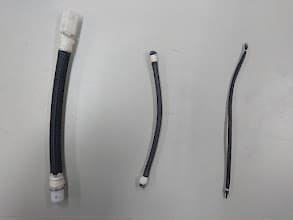
\includegraphics[scale=0.7]{image/hikaku.jpg}
  \caption{MPAの外径の比較(左から12,5,3 mm)}
  \label{fig:campare}
\end{figure}
%
\begin{figure}
  %
  \begin{minipage}[b]{0.49\columnwidth}
    \centering  
    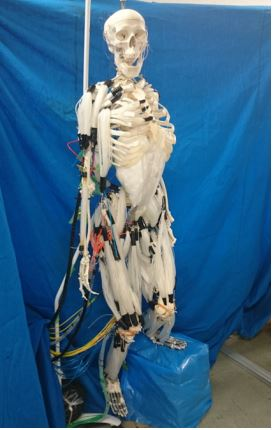
\includegraphics[scale=0.5]{image/kinkokkaku.JPG}
    \subcaption{筋骨格系ロボット\cite{森田隆介2016}}
    \label{fig:kin}
  \end{minipage}
  %
  \begin{minipage}[b]{0.49\columnwidth}
    \centering
    \vspace{5mm}
    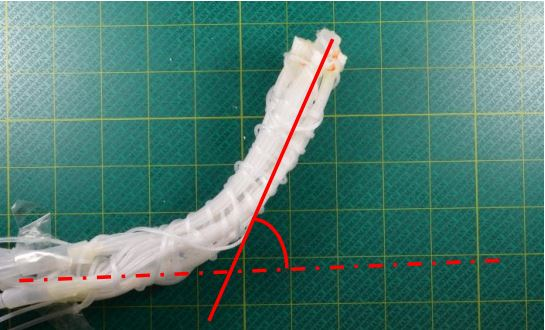
\includegraphics[scale=0.5]{image/takoJPG.JPG}
    \subcaption{タコ腕模倣メカニズム\cite{森和也2014}}
    \label{fig:tako}
  \end{minipage}
  %
  \caption{細径空圧筋を用いたロボット}
  \label{fig:saikei}
\end{figure}
%%
\begin{figure}[t]
  \centering
  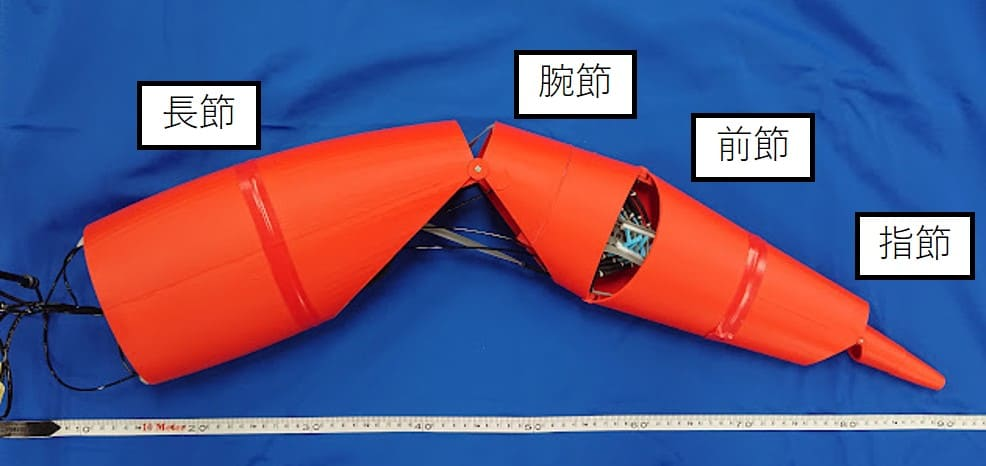
\includegraphics[scale=0.3]{image/robot_scale.JPG}
  \vspace{3mm}
  \caption{先行研究で作製された歩脚ロボット\cite{hasegawa}}
  \label{fig:senkoukenkyuu}
\end{figure}
  %
\begin{figure}[t]
  \centering
  \vspace{3mm}
  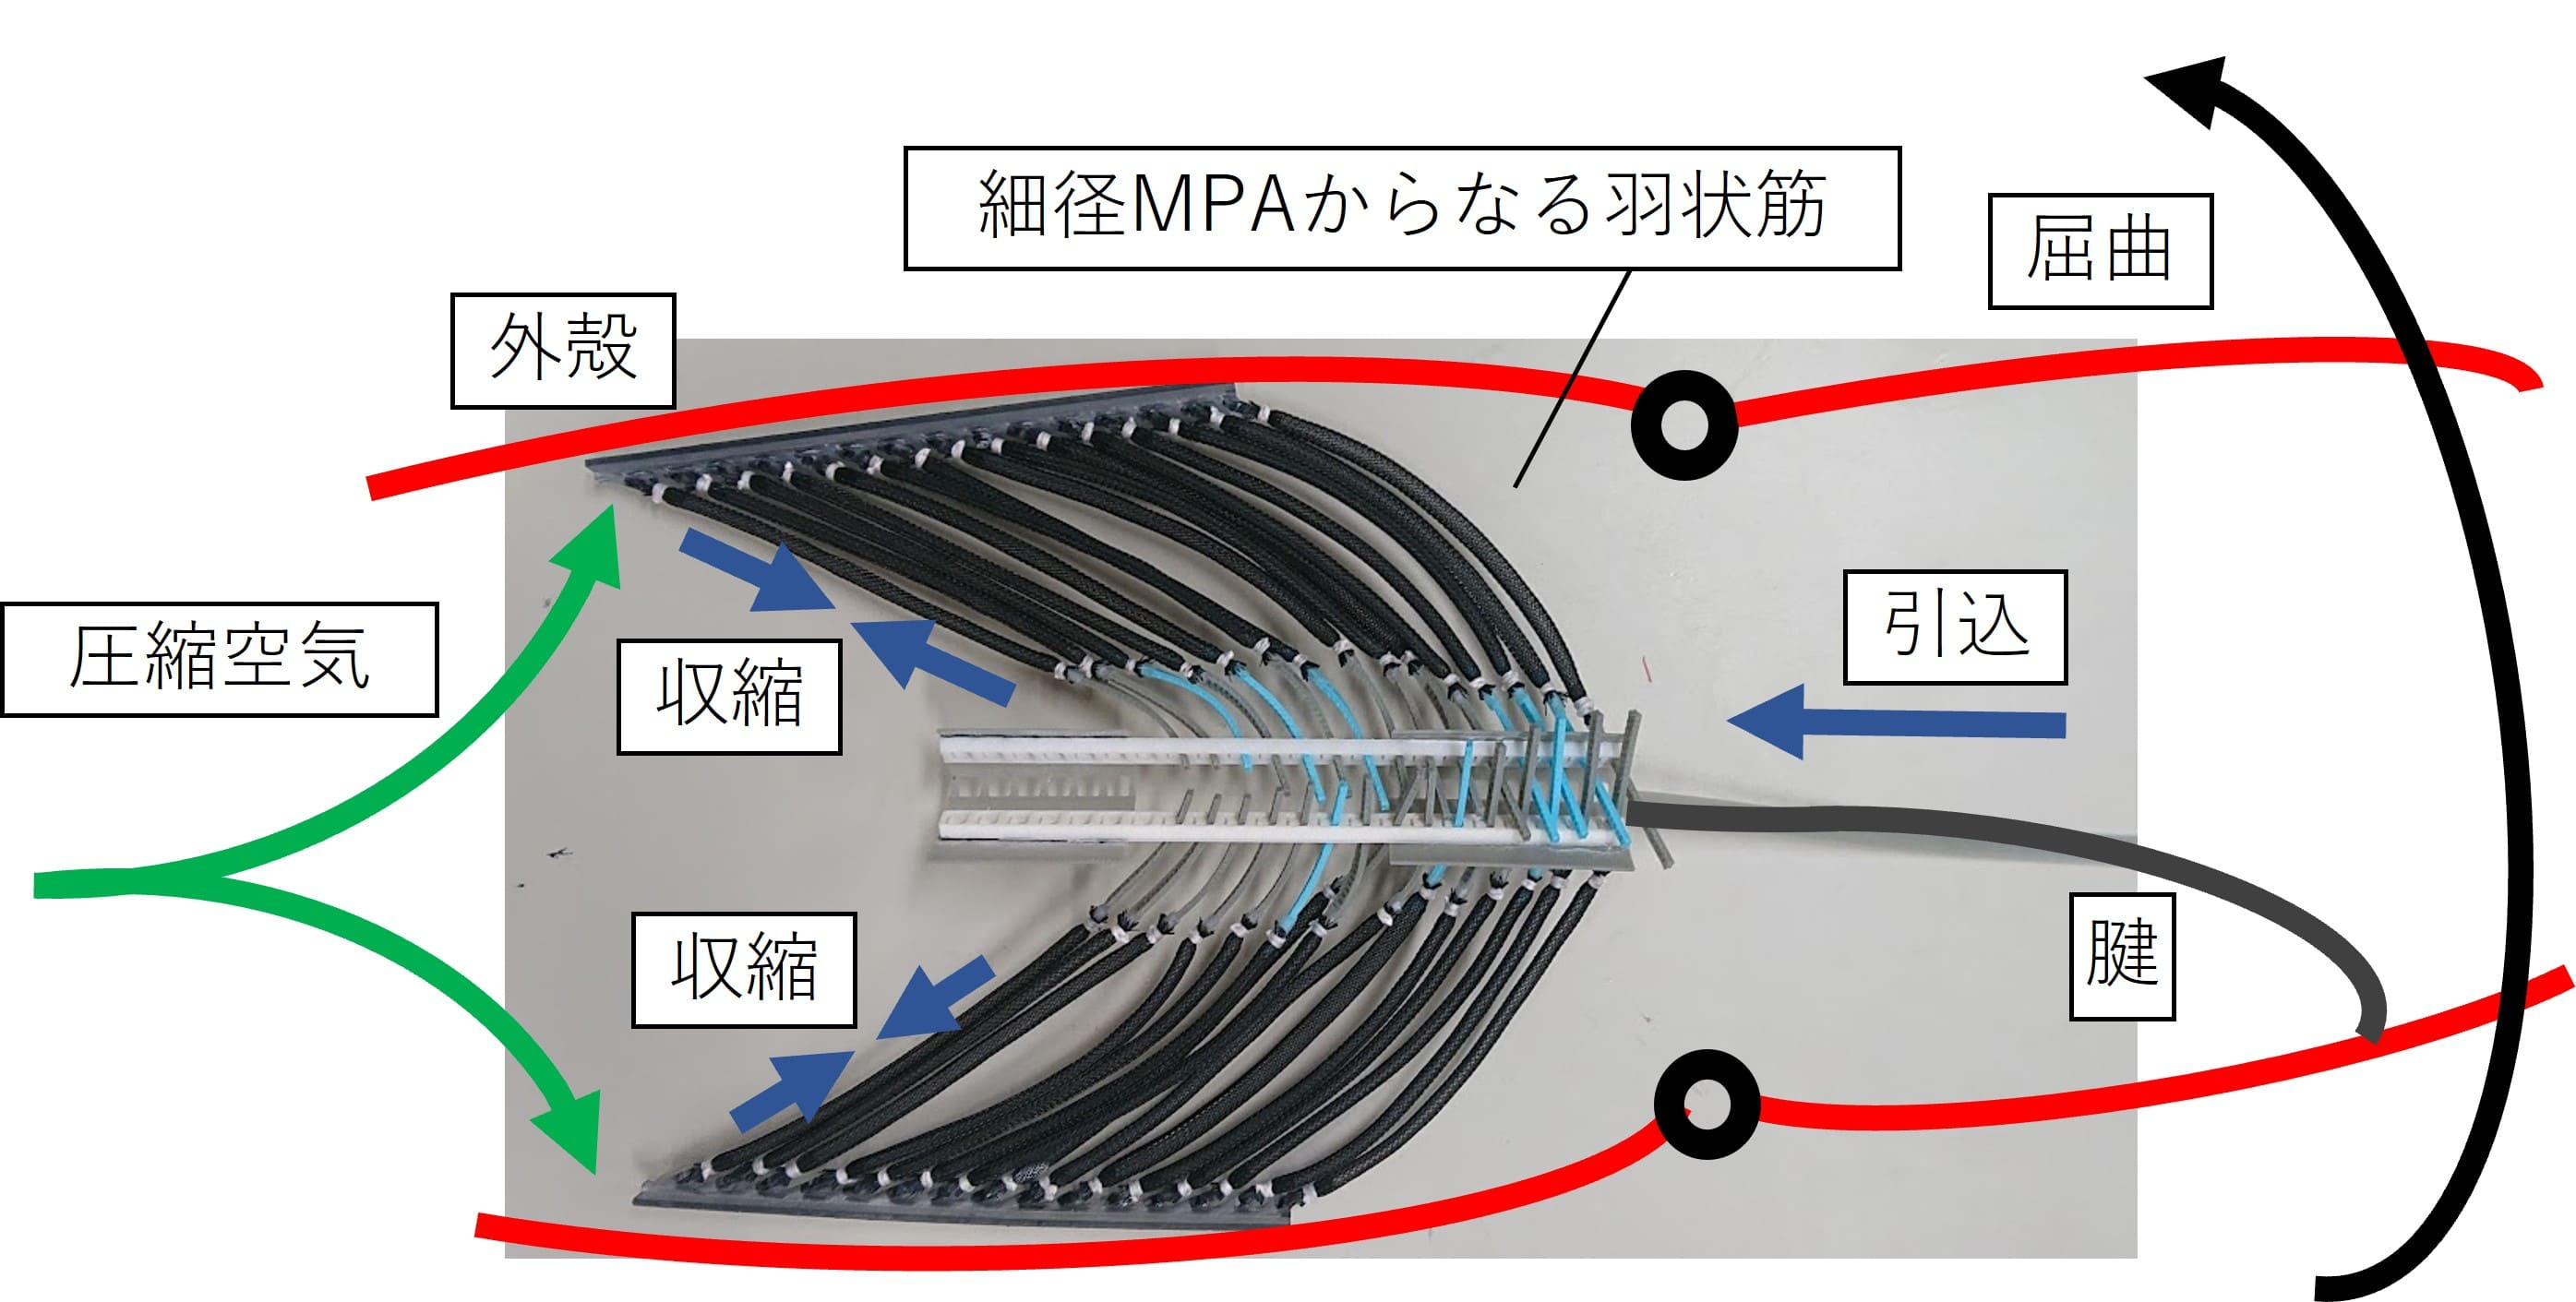
\includegraphics[scale=0.14]{image/mosiki.JPG}
  \caption{先行研究で開発された羽状筋\cite{hasegawa}}
  \label{fig:ujyoukin}
\end{figure}
%%
\begin{figure}[tbp]
  \begin{minipage}{1\hsize}
    \centering
    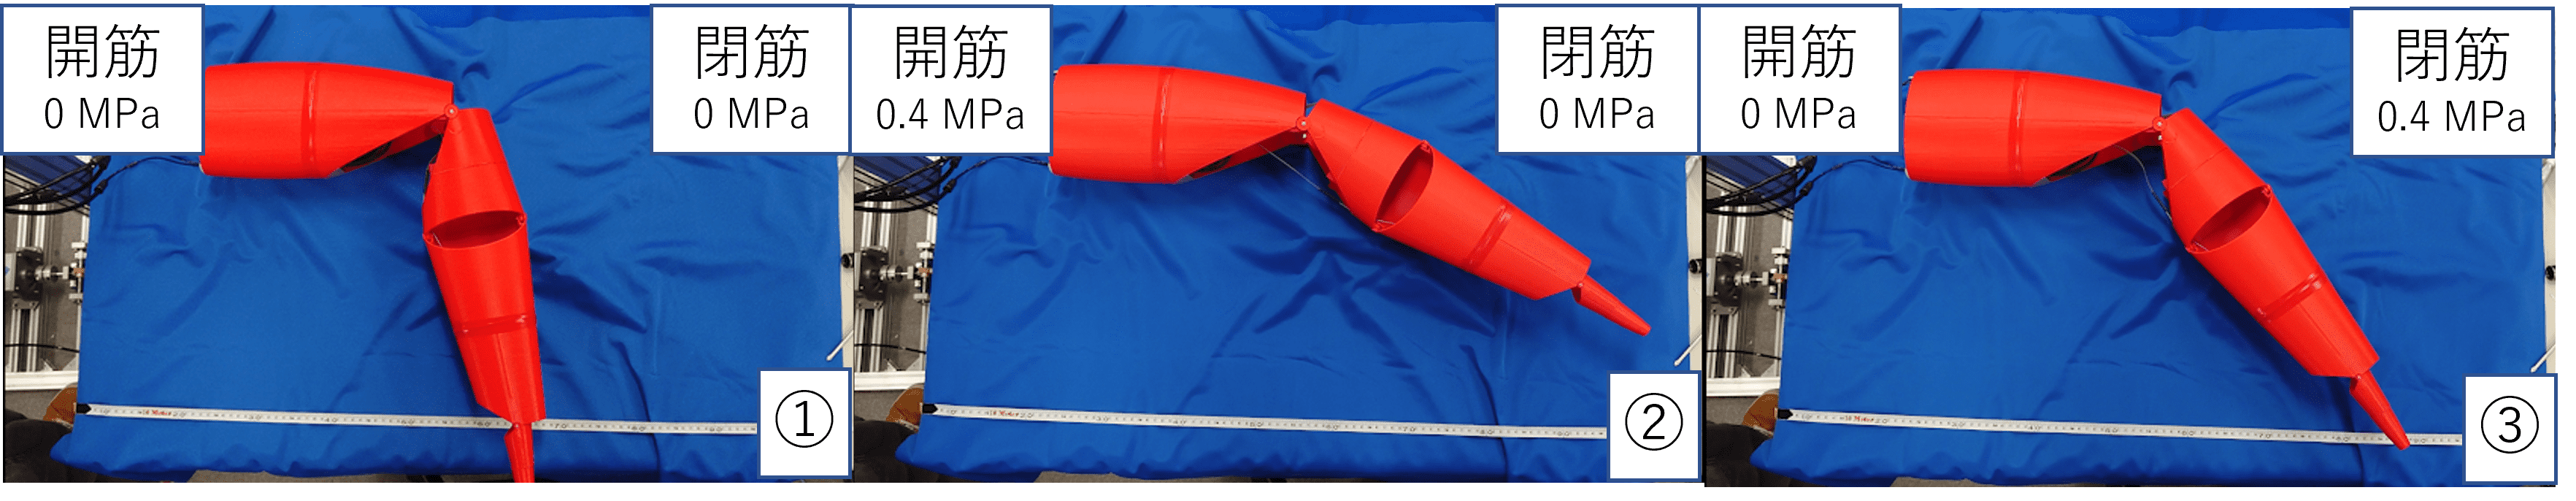
\includegraphics[scale=0.12]{image/move1all.png}
    \subcaption{長節-腕節間の動作\cite{hasegawa}}
    \label{fig:move1}
  \end{minipage}
  %
  \begin{minipage}{1\hsize}
    \centering
    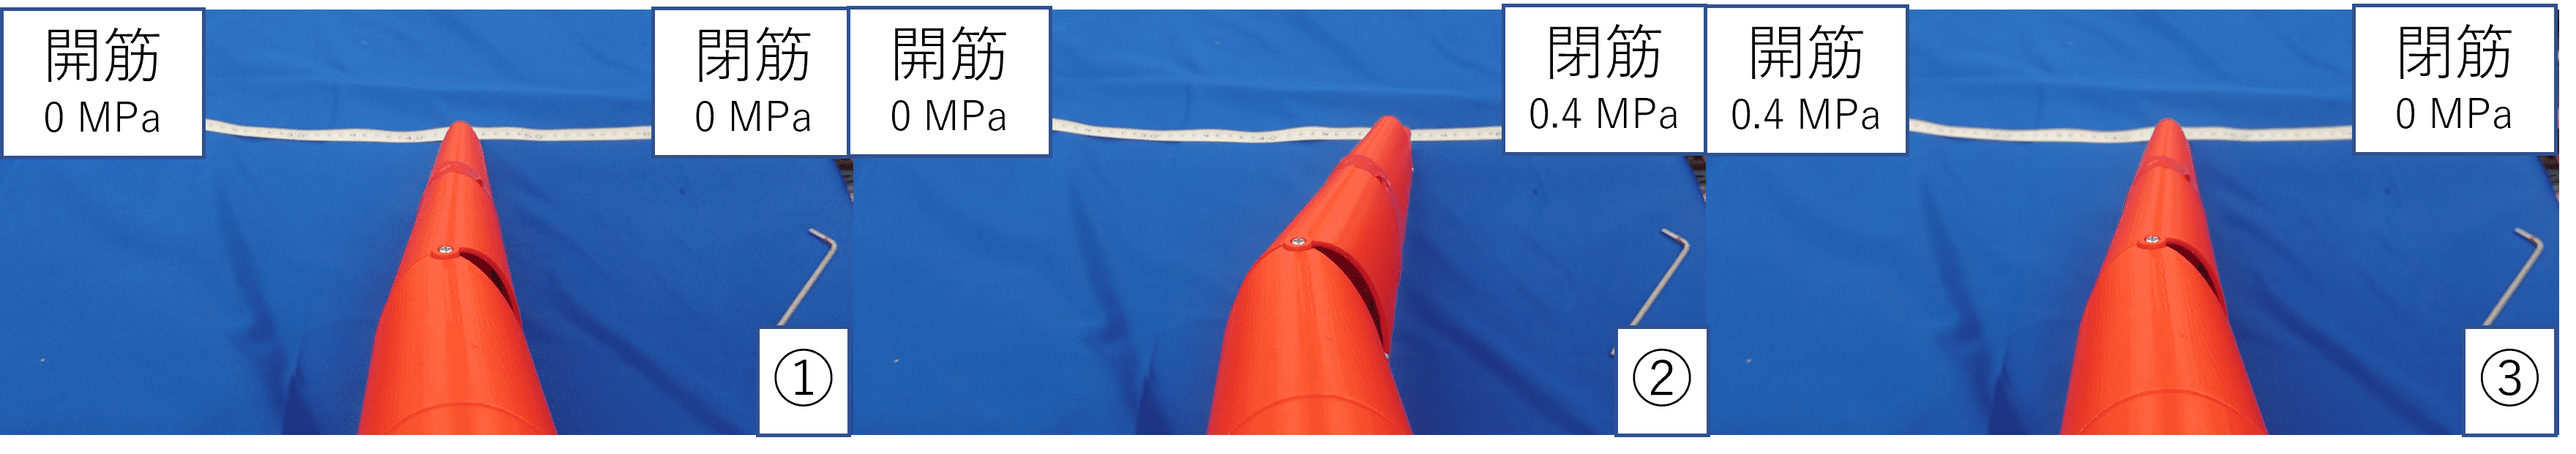
\includegraphics[scale=0.12]{image/move2all.png}
    \subcaption{腕節-前節間の動作\cite{hasegawa}}
    \label{fig:move2}
  \end{minipage}
%
  \caption{動作実験}
  \label{fig:movea12}
\end{figure}
%
%%%%%%%%%%%%%%%%%%%%%%%%%%%%%%%%%%%%%%%%%%%%%%%%%%%%%%%%%
\subsection{先行研究の成果と課題}
先行研究\cite{hasegawa}では図\ref{fig:senkoukenkyuu}のような歩脚ロボットの作製に成功した.このロボットでは図\ref{fig:ujyoukin}のように細径MPAを用いて蟹の羽のような構造である羽状筋と呼ばれる筋肉を再現することができた\cite{hasegawa}.
このロボットで動作実験を行い図\ref{fig:movea12}のように開閉動作をすることを確認することができた.

しかし,以下のような課題点が見つかった
\begin{enumerate}
  \item 細径MPAの作製方法が煩雑で時間がかかり,技術も必要
  \item 細径MPAの収縮性能が低く,腱を充分に引き込めない
  \item 細径MPAの根元部分の角度が固定されており,腱の引き込みを妨げている
\end{enumerate}
そこで本研究では,上記のような先行研究で見つかった課題点を解決した細径MPAおよび羽状筋さらに歩脚ロボットの開発に取り組む.
            % 本文
%\newpage
\section{モデル生物の構成および筋構造}
本章では今回モデルにする甲殻類の蟹について,外骨格と内骨格の違いや本研究で重要となる筋構造など実際にズワイガニを解剖した知見なども基に述べる.
%%%%%%%%%%%%%%%%%%%%%%%%%%%%%%%%%%%%%%%%%%%%%%%%%%%%%%%%%
\subsection{使用したモデル生物}
\subsubsection{外骨格}
%%%%%%%%%%%%%%%%%%%%%%%%%%%%%%%%%%%%%%%%%%%%%%%%%%%%%%%%%
\subsubsection{羽状筋}
%%%%%%%%%%%%%%%%%%%%%%%%%%%%%%%%%%%%%%%%%%%%%%%%%%%%%%%%%
\subsubsection{蟹の関節の可動域}
%%%%%%%%%%%%%%%%%%%%%%%%%%%%%%%%%%%%%%%%%%%%%%%%%%%%%%%%%
\subsection{外骨格の設計方法}
\subsubsection{外骨格の寸法}
%%%%%%%%%%%%%%%%%%%%%%%%%%%%%%%%%%%%%%%%%%%%%%%%%%%%%%%%%
\subsubsection{機体の可動域計算に用いた簡易モデル}
%%%%%%%%%%%%%%%%%%%%%%%%%%%%%%%%%%%%%%%%%%%%%%%%%%%%%%%%%
\begin{figure}[b]
    \begin{minipage}{0.49\hsize}
      \vspace{15mm}
      \centering
      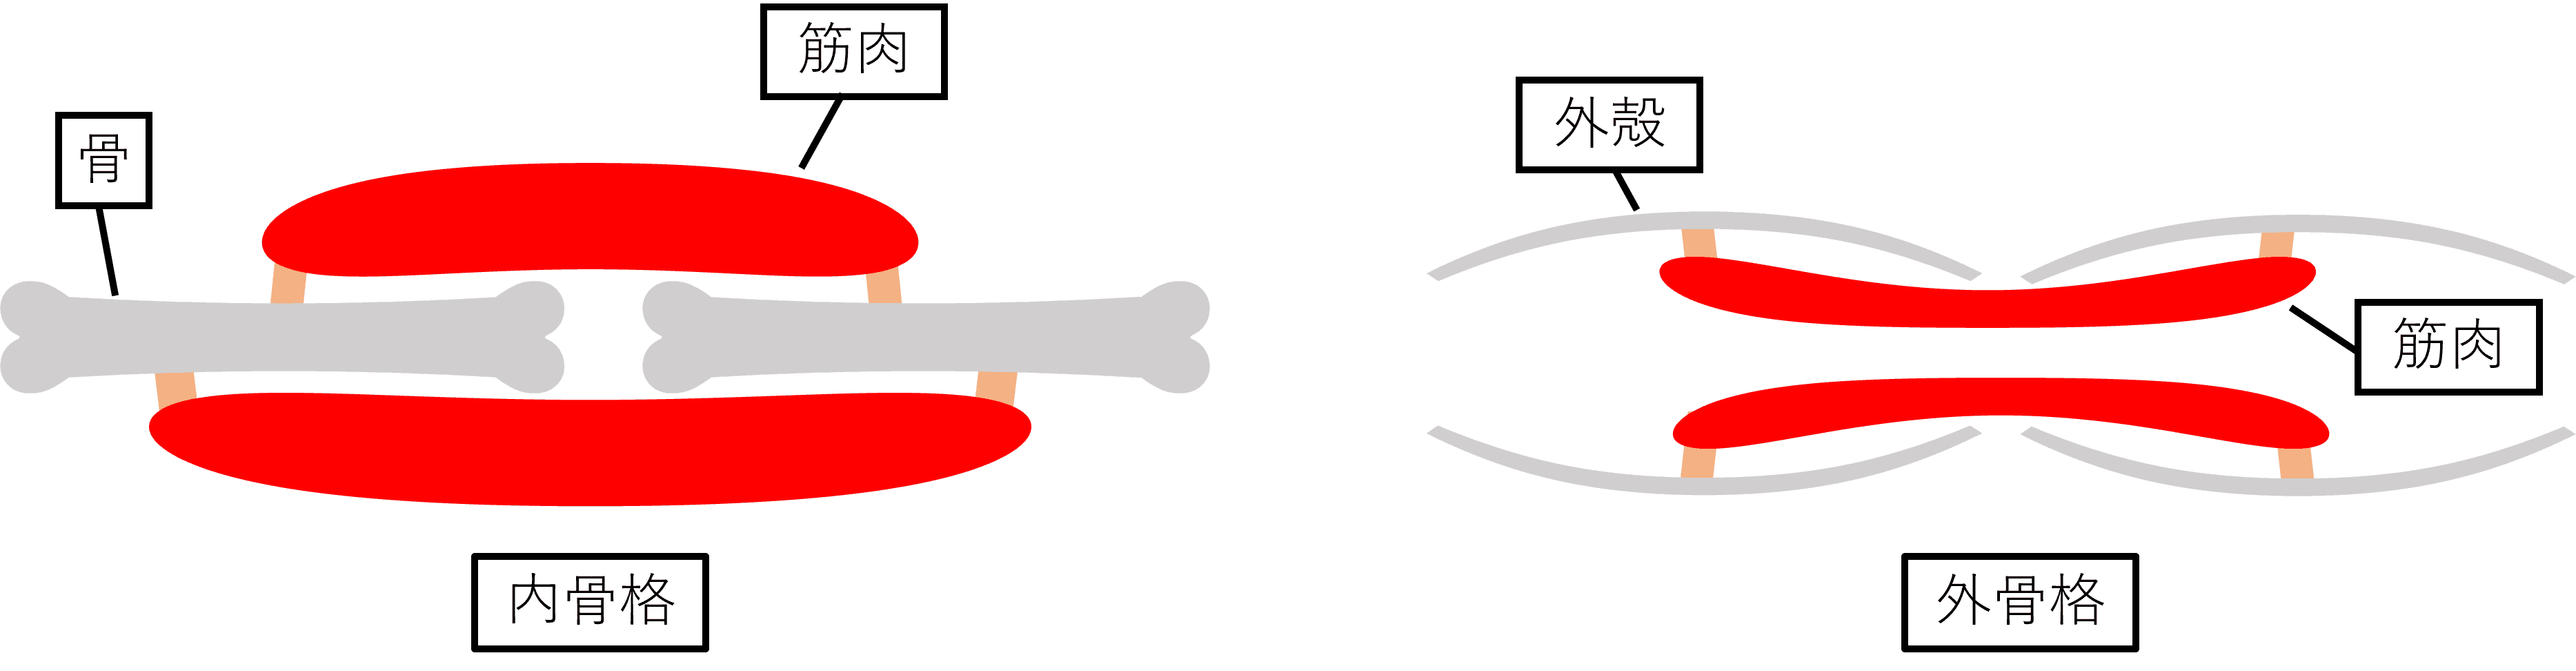
\includegraphics[scale=0.058]{image/kokkaku.png}
      \caption{内骨格と外骨格}
      \label{fig:naigai}
    \end{minipage}
    %
    \begin{minipage}{0.49\hsize}
      \centering
      \includegraphics[scale=.05]{image/apearance3_1.png}
      \caption{解剖に用いたズワイガニ}
      \label{fig:zuwai}
    \end{minipage}
\end{figure}
%%%%%%%%%%%%%%%%%%%%%%%%%%%%%%%%%%%%%%%%%%%%%%%%%%%%%%%%%
\begin{table}[htbp]
  \centering
  \caption{第1肢の長節から指節の寸法}
  \label{tab:1setu}
  \vspace{-3mm}
  \begin{tabular}{|l|c|c|c|c|c|}
  \hline
     & \multicolumn{1}{l|}{幅-左 [mm]} & \multicolumn{1}{l|}{幅-中 [mm]} & \multicolumn{1}{l|}{幅-右 [mm]} & \multicolumn{1}{l|}{厚み [mm]} & \multicolumn{1}{l|}{長さ [mm]} \\ \hline
  長節 & 12.01                       & 12.01                       & 8.86                        & 7.68                        & 52.0                        \\ \hline
  腕節 & 6.11                        & -                           & 9.85                        & 7.60                        & 14.5                        \\ \hline
  前節 & 10.39                       & -                           & 7.12                        & 4.26                        & 38.0                        \\ \hline
  指節 & -                           & 4.51                        & -                           & 3.36                        & 24.5                        \\ \hline
  \end{tabular}
\end{table}
%
\begin{table}[htbp]
  \centering
  \caption{第2肢の長節から指節の寸法}
  \label{tab:2setu}
  \vspace{-3mm}
  \begin{tabular}{|l|c|c|c|c|c|}
  \hline
     & \multicolumn{1}{l|}{幅-左 [mm]} & \multicolumn{1}{l|}{幅-中 [mm]} & \multicolumn{1}{l|}{幅-右 [mm]} & \multicolumn{1}{l|}{厚み [mm]} & \multicolumn{1}{l|}{長さ [mm]} \\ \hline
  長節 & 18.10                       & 19.05                       & 11.85                       & 9.18                        & 87.5                        \\ \hline
  腕節 & 8.59                        & -                           & 16.14                       & 7.32                        & 27.5                        \\ \hline
  前節 & 16.14                       & -                           & 8.83                        & 4.40                        & 58.5                        \\ \hline
  指節 & -                           & 5.43                        & -                           & 2.65                        & 25.0                        \\ \hline
  \end{tabular}
\end{table}
%
\begin{table}[htbp]
  \centering
  \caption{第3肢の長節から指節の寸法}
  \label{tab:3setu}
  \vspace{-3mm}
  \begin{tabular}{|l|c|c|c|c|c|}
  \hline
     & \multicolumn{1}{l|}{幅-左 [mm]} & \multicolumn{1}{l|}{幅-中 [mm]} & \multicolumn{1}{l|}{幅-右 [mm]} & \multicolumn{1}{l|}{厚み [mm]} & \multicolumn{1}{l|}{長さ [mm]} \\ \hline
  長節 & 18.38                       & 20.88                       & 13.56                       & 9.98                        & 102.0                       \\ \hline
  腕節 & 9.70                        & -                           & 17.30                       & 9.12                        & 31.5                        \\ \hline
  前節 & 17.06                       & -                           & 9.01                        & 4.91                        & 63.5                        \\ \hline
  指節 & -                           & 5.62                        & -                           & 3.93                        & 27.5                        \\ \hline
  \end{tabular}
\end{table}
%
\begin{table}[htbp]
  \centering
  \caption{第4肢の長節から指節の寸法}
  \label{tab:4setu}
  \vspace{-3mm}
  \begin{tabular}{|l|c|c|c|c|c|}
  \hline
     & \multicolumn{1}{l|}{幅-左 [mm]} & \multicolumn{1}{l|}{幅-中 [mm]} & \multicolumn{1}{l|}{幅-右 [mm]} & \multicolumn{1}{l|}{厚み [mm]} & \multicolumn{1}{l|}{長さ [mm]} \\ \hline
  長節 & 19.10                       & 21.74                       & 13.11                       & 11.05                       & 100.0                       \\ \hline
  腕節 & 10.57                       & -                           & 18.42                       & 8.74                        & 40.5                        \\ \hline
  前節 & 16.48                       & -                           & 10.40                       & 4.68                        & 70.0                        \\ \hline
  指節 & -                           & 5.60                        & -                           & 3.69                        & 30.0                        \\ \hline
  \end{tabular}
  \end{table}
  %
  \begin{table}[htbp]
    \centering
    \caption{第5肢(鋏脚)の長節から指節の寸法}
    \label{tab:5setu}
    \vspace{-3mm}
    \begin{tabular}{|c|c|c|c|}
    \hline
    \multicolumn{1}{|l|}{} & \multicolumn{1}{l|}{幅(左-中-右) {[}mm{]}} & \multicolumn{1}{l|}{厚み(左-中-右) {[}mm{]}} & \multicolumn{1}{l|}{長さ [mm]} \\ \hline
    長節                     & 18.10-18.23-18.24                     & 11.72-15.05-15.89                      & 63.5                        \\ \hline
    腕節                     & 11.70-18.40-19.31                     & 13.23-18.64-17.03                      & 15.5                        \\ \hline
    前節                     & 22.97-25.82-25.06                     & 14.75-21.30-19.09                      & 50.0                        \\ \hline
    前節(鋏部)                 & 8.64----                              & ----4.45                          & 45.0                      \\ \hline
    指節                     & 8.15----                              & ----4.26                               & 50.0                        \\ \hline
    \end{tabular}
  \end{table}
  %
  \begin{table}[htbp]
  \begin{minipage}{0.5\hsize}
    \centering
    \caption{第1肢の節間の可動域}
    \label{tab:1kadou}
    \vspace{-3mm}
    \begin{tabular}{|l|c|}
    \hline
       & \multicolumn{1}{l|}{可動域 [deg]} \\ \hline
    長節-腕節間 & 0-155                         \\ \hline
    腕節-前節間 & 0-81                          \\ \hline
    前節-指節間 & 0-110                         \\ \hline
    \end{tabular}
  \end{minipage}
  %
  \begin{minipage}{0.5\hsize}
    \centering
    \caption{第2肢の節間の可動域}
    \label{tab:2kadou}
    \vspace{-3mm}
    \begin{tabular}{|l|c|}
    \hline
       & \multicolumn{1}{l|}{可動域 [deg]} \\ \hline
    長節-腕節間 & 0-145                         \\ \hline
    腕節-前節間 & 0-50                          \\ \hline
    前節-指節間 & 0-90                          \\ \hline
    \end{tabular}
  \end{minipage}
  %
  \begin{minipage}{0.5\hsize}
    \centering
    \vspace{5mm}
    \caption{第3肢の節間の可動域}
    \label{tab:3kadou}
    \vspace{-3mm}
    \begin{tabular}{|l|c|}
    \hline
       & \multicolumn{1}{l|}{可動域 [deg]} \\ \hline
    長節-腕節間 & 0-150                         \\ \hline
    腕節-前節間 & 0-45                          \\ \hline
    前節-指節間 & 0-80                          \\ \hline
    \end{tabular}
  \end{minipage}
  %
  \begin{minipage}{0.5\hsize}
    \centering
    \vspace{5mm}
    \caption{第4肢の節間の可動域}
    \label{tab:4setukadou}
    \vspace{-3mm}
    \begin{tabular}{|l|c|}
    \hline
           & \multicolumn{1}{l|}{可動域 {[}deg{]}} \\ \hline
    長節-腕節間 & 0-140                            \\ \hline
    腕節-前節間 & 0-45                             \\ \hline
    前節-指節間 & 0-89                            \\ \hline
    \end{tabular}
  \end{minipage}
\end{table}
%
\begin{table}[htbp]
  \centering
  \vspace{5mm}
  \caption{第5肢の節間の可動域}
  \label{tab:5kadou}
  \vspace{-3mm}
  \begin{tabular}{|l|c|}
  \hline
         & \multicolumn{1}{l|}{可動域 [deg]} \\ \hline
  長節-腕節間 & 70-140                        \\ \hline
  腕節-前節間 & 0-40                          \\ \hline
  前節-指節間 & 15-30                         \\ \hline
  \end{tabular}
  \end{table}
%%%%%%%%%%%%%%%%%%%%%%%%%%%%%%%%%%%%%%%%%%%%%%%%%%%%%%%%%
\begin{figure}[t]
%
  \begin{minipage}{1\hsize}
    \centering
    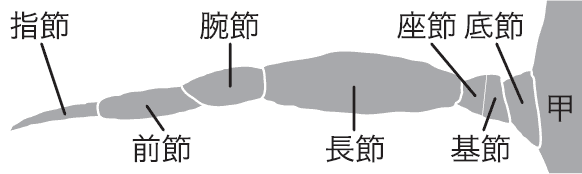
\includegraphics[scale=0.52]{image/setu.PNG}
    \caption{節の名称\cite{crabnature}}
    \vspace{3mm}
    \label{fig:setu}
  \end{minipage}
%
  \begin{minipage}{1\hsize}
    \centering
    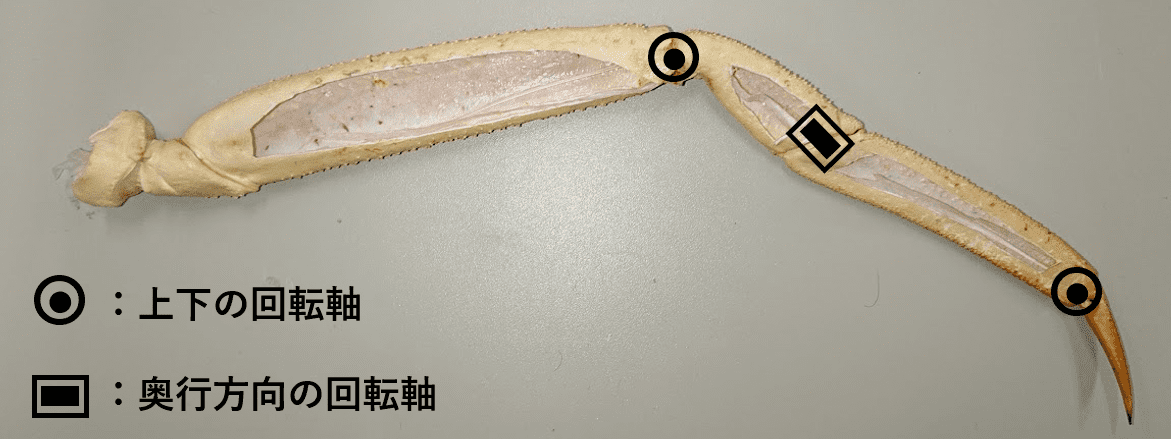
\includegraphics[scale=0.26]{image/kaiten.png}
    \caption{ズワイガニの脚の可動域}
    \label{fig:kaiten}
  \end{minipage}
  %
  \begin{minipage}{0.5\hsize}
    \centering
    \vspace{3mm}
    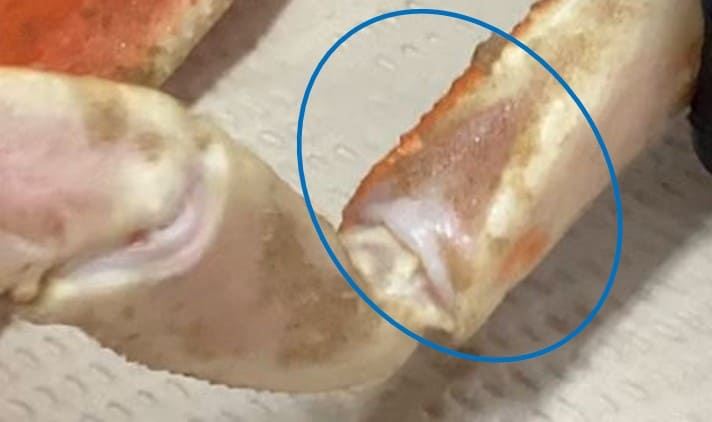
\includegraphics[scale=0.24]{image/maku1.JPG}
    \caption{節間膜}
    \label{fig:maku}
  \end{minipage}
%
    \begin{minipage}{0.5\hsize}
      \centering
      \vspace{4mm}
      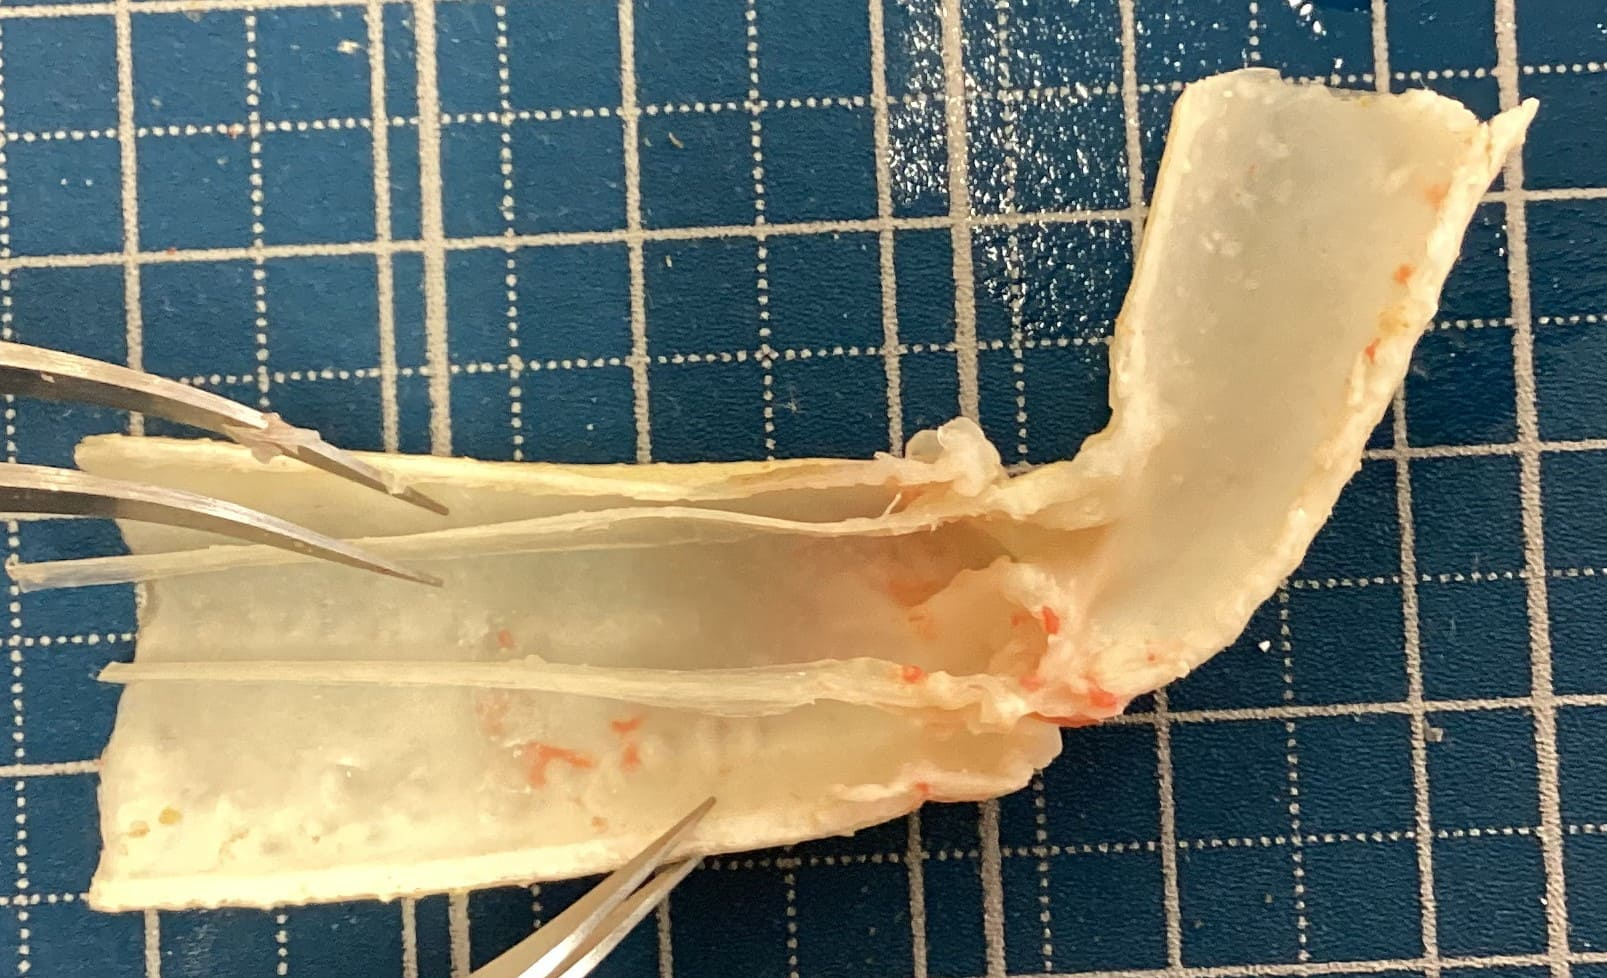
\includegraphics[scale=0.1]{image/setukanmaku.jpg}
      \caption{腱の様子}
      \label{fig:ken}
    \end{minipage}
  \end{figure}
%%%%%%%%%%%%%%%%%%%%%%%%%%%%%%%%%%%%%%%%%%%%%%%%%%%%%%%%%
\vspace{15mm}
\subsection{蟹の関節構造と筋構造および筋配置}
\subsubsection{関節構造}
蟹の脚は鋏脚と歩脚の5対10本から構成され,それぞれの脚は甲に近いほうから底節,基節,座節,長節,腕節,前節,指節の7つの節からなる(図\ref{fig:setu}).基節,座節の間の関節は融合し1つの節のように見える場合もある\cite{crabnature}.
脚を構成する7つの節が接する関節の部分はそれぞれ動く方向が決まっており,底節は複雑に配置された筋によって前後左右に動かすことが可能であるが,それよりも遠位の関節は基本的には単純な開閉動作をする.
図\ref{fig:kaiten}に解剖したズワイガニの歩脚に回転軸を追記したものを示す.
今回用いるズワイガニに関しては長節から指節のうち,腕節-前節間は前後に可動域を持つが,それ以外の節間は甲から腹側への開閉方向の可動域を持つことが分かった.
また,それぞれの節間には節間膜と呼ばれる丈夫で柔軟なクチクラ質の組織によって繋がっている(図\ref{fig:maku}).
%%%%%%%%%%%%%%%%%%%%%%%%%%%%%%%%%%%%%%%%%%%%%%%%%%%%%%%%%
\subsubsection{筋構造}
蟹の脚の筋肉について,蟹の脚内部を充填する筋繊維の一端は節の内壁に付着し,もう一方は腱と呼ばれる組織,いわゆる蟹のすじに付着する.
腱は隣の関節の端に繋がっており,筋繊維が収縮することによって腱が引っ張られ節が開閉する.
ズワイガニを解剖した際に記録した長節-腕節間の腱の様子を図\ref{fig:ken}に示す.
解剖結果よりズワイガニの腱は節間膜と一体になるように挿入されていることが分かった.
筋繊維は腱に対して斜めに充填されており,このように配置された筋繊維を羽状筋という.
羽状筋の動きの模式図を図\ref{fig:ujo}に示す.
羽状筋には2つの利点があるとされている.1つ目は収縮しても膨張せず,羽状筋の角度が大きくなるだけなので限られた狭い空間で働くのに適していること,2つ目は同じ形状と体積の平行筋と比べ収縮時に約2倍の力を発揮することが出来ることである\cite{warner1977biology}.
%%%%%%%%%%%%%%%%%%%%%%%%%%%%%%%%%%%%%%%%%%%%%%%%%%%%%%%%%
\subsubsection{筋配置}
脚内部の筋肉配置について,同じく十脚目短尾下目のLibinia emarginataの歩脚と鋏脚の筋構造を図\ref{fig:libinia}に,ヨーロッパイチョウガニとヨーロッパミドリガニの歩脚をCTスキャンしたものを図\ref{fig:ct}\subref{fig:ct1},\subref{fig:ct2}に示す.
図\ref{fig:libinia},図\ref{fig:ct}より,3種の歩脚の長節以降の筋配置は非常に似ていることが分かり,腕節-前節間,前節-指節間は節の可動域に沿って配置されているが,長節-腕節間は可動域よらず縦に配置されている.
また,図\ref{fig:libinia}より,底節,基節,座節部分は複雑な筋配置となっていることが分かる.
本研究ではズワイガニの長節-指節間の筋配置はこれらと同様なものとして扱い,節を開く方向に作用する羽状筋を開筋,閉じる方向へと作用するものを閉筋とする.
また,筋配置が複雑な底節,基節,座節は扱わないものとする.
%%%%%%%%%%%%%%%%%%%%%%%%%%%%%%%%%%%%%%%%%%%%%%%%%%%%%%%%%
\begin{figure}[t]
  \begin{minipage}{1\hsize}
    \centering
    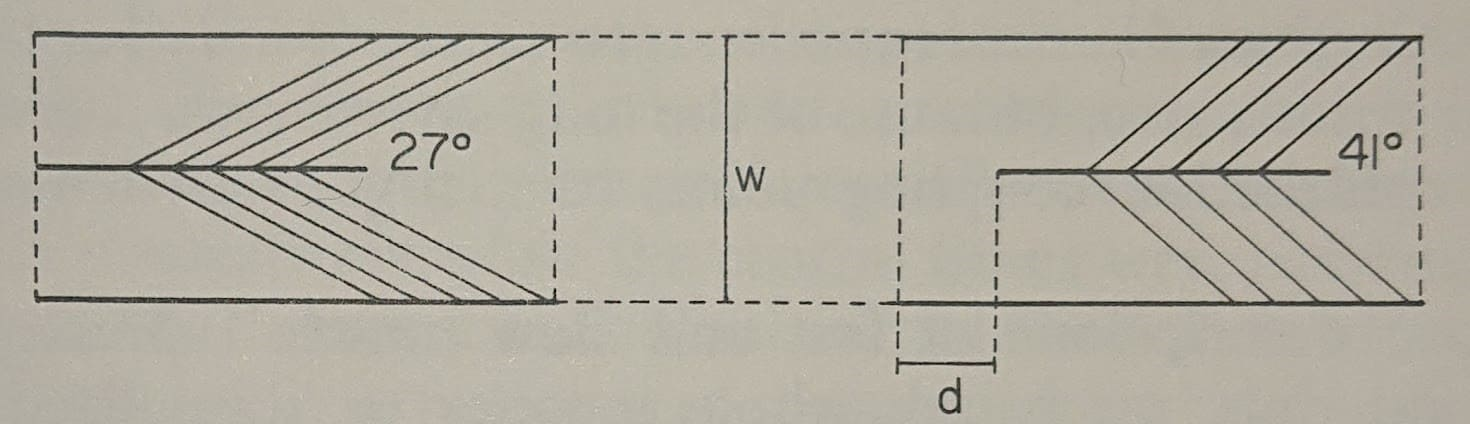
\includegraphics[scale=0.3]{image/ujo.JPG}
    \caption{羽状筋の動きを模式的に表したもの.左側が筋肉が伸展,右側が収縮した状態.収縮中,羽状筋の角度は27 degから41 degに増加し,腱は距離dを移動する.各筋繊維は短く太くなるが,筋全体の幅wは変化しない\cite{warner1977biology}}
   \label{fig:ujo}
  \end{minipage}
\end{figure}
  
\begin{figure}[t]
  \centering
  \vspace{-3mm}
  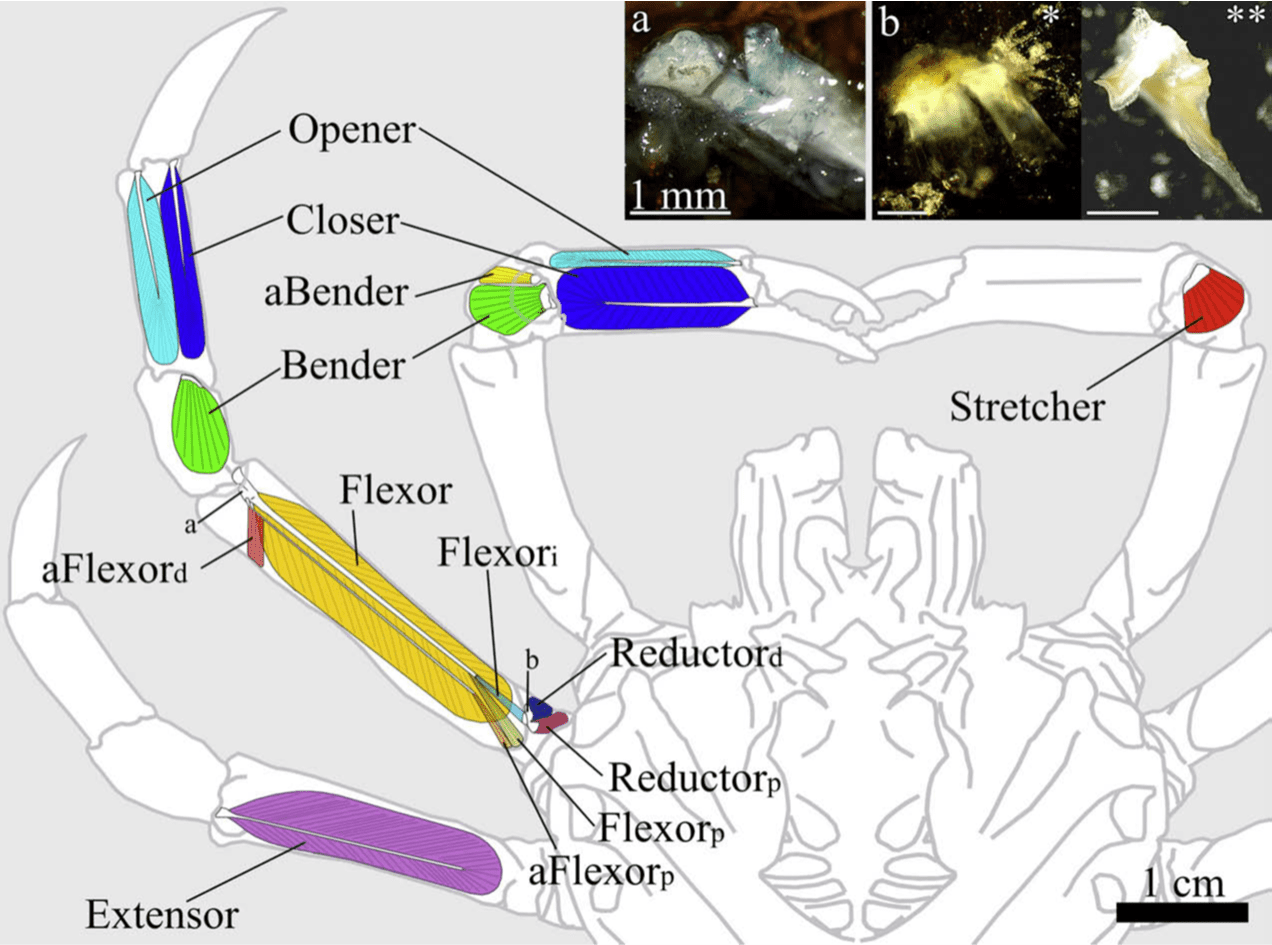
\includegraphics[scale=0.25]{image/libinia.png}
  \caption{Libinia emarginataの歩脚と鋏脚の筋構造\cite{VIDALGADEA2009179}}
  \label{fig:libinia}
\end{figure}
%
\begin{figure}[t]
%
  \begin{minipage}{0.45\hsize}
    \centering
    \vspace{5mm}
    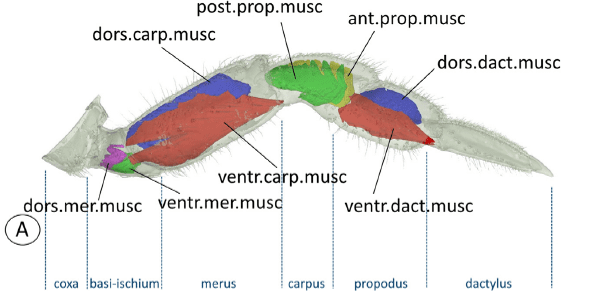
\includegraphics[scale=0.5]{image/crabct2.PNG}
    \subcaption{ヨーロッパイチョウガニ}
    % \vspace{3mm}
    \label{fig:ct1}
  \end{minipage}
  %
  \begin{minipage}{0.45\hsize}
    \centering
    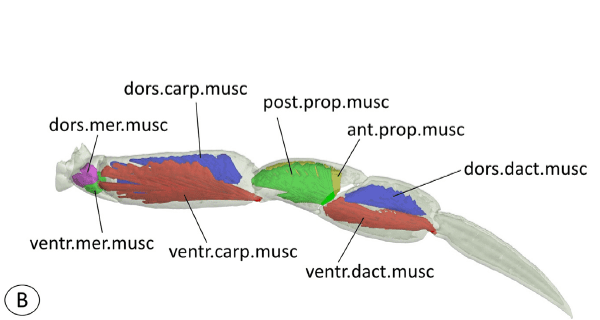
\includegraphics[scale=0.5]{image/crabct1.PNG}
    \subcaption{ヨーロッパミドリガニ}
    % \vspace{3mm}
    \label{fig:ct2}
  \end{minipage}
  \caption{歩脚のctスキャン画像\cite{HAZERLI2020100972}}
  \label{fig:ct}
%
\end{figure}
%%%%%%%%%%%%%%%%%%%%%%%%%%%%%%%%%%%%%%%%%%%%%%%%%%%%%%%%%






%\newpage
\section{改良型細径羽状筋の開発}
本章では,先行研究\cite{hasegawa}において開発された羽状筋に関する3つの課題点について,どのように解決を行ったかを述べる.
%%%%%%%%%%%%%%%%%%%%%%%%%%%%%%%%%%%%%%%%%%%%%%%%%%%%%%%%%
\subsection{先行研究で確認された課題}
\subsection{課題1:細径MPAの制作方法の改良}
先行研究の細径MPA締結方法を図\ref{fig:MPA_tanbu_1}に示す.先行研究では,細径MPAを構成するシリコンチューブとスリーブを端部で糸で縛り接着剤で固定する方式を採用していた.
しかし,この方法では作製するのに時間がかかる.また,空気漏れが生じてしまい,完成するのに技術と練度が必要となる.
そこで本研究では,図\ref{fig:MPA_tanbu_2}のように細径MPA端部部品とOリングを用いた新しい細径MPA作製方法を開発した.
新型細径MPAの作製手順を以下に示す.従来の細径MPA作製方法を用いると作製時間が約20分なのに対し,本研究の作製方法では約10分で作製することが可能であり,空気漏れなどの が発生する確率も大幅に低くなった.
\vspace{3mm}
\begin{enumerate}
  \item 図\ref{fig:MPA_tanbu_2_2}のようにゴムチューブを端部部品の溝部分に差し込み,差し込んだ隙間に接着剤を塗布する
  \item 接着剤が乾いたら,図\ref{fig:MPA_tanbu_2_1}のようにゴムチューブと端部部品をスリーブで包む
  \item 図\ref{fig:MPA_tanbu_2_1}のように図\ref{fig:MPA_tanbu_2_2}中のOリング固定溝にはまるようにOリングを配置する
  \item 端部部品,スリーブとOリングを固定するために接着剤を塗布する
\end{enumerate}
%%%%%%%%%%%%%%%%%%%%%%%%%%%%%%%%%%%%%%%%%%%%%%%%%%%%%%%%%
\begin{figure}[!hb]
  %
  \begin{minipage}{0.49\hsize}
    \centering  
    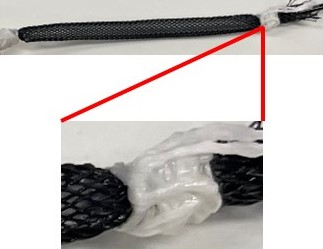
\includegraphics[scale=0.4]{image/MPA_tanbu_1_1.jpg}
    \subcaption{旧型細径MPA外観}
    \label{fig:MPA_tanbu_1_1}
  \end{minipage}
  %
  \begin{minipage}{0.5\hsize}
    \centering
    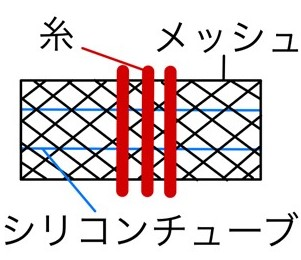
\includegraphics[scale=0.4]{image/MPA_tanbu_1_2.jpg}
    \subcaption{旧型細径MPA模式図}
    \label{fig:MPA_tanbu_1_2}
  \end{minipage}
  %
  \caption{先行研究で用いられた旧型細径MPAおよび作製方法}
  \label{fig:MPA_tanbu_1}
\end{figure}
%
\begin{figure}[!hb]
  \begin{minipage}{0.49\hsize}
    \centering
    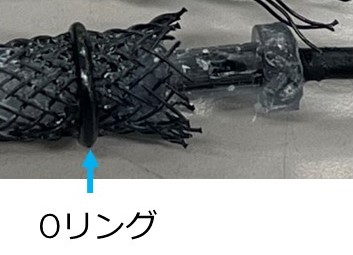
\includegraphics[scale=0.4]{image/MPA_tanbu_2_2.jpg}
    \subcaption{新型細径MPA外観}
    \label{fig:MPA_tanbu_2_1}
  \end{minipage}
  %
  \begin{minipage}{0.49\hsize}
    \centering  
    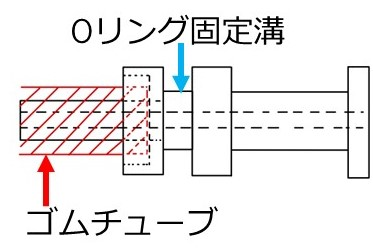
\includegraphics[scale=0.4]{image/MPA_tanbu_2_1.jpg}
    \subcaption{新型細径MPA模式図}
    \label{fig:MPA_tanbu_2_2}
  \end{minipage}
  \caption{本研究で用いた新型細径MPAおよび作製方法}
  \label{fig:MPA_tanbu_2}
\end{figure}
%%%%%%%%%%%%%%%%%%%%%%%%%%%%%%%%%%%%%%%%%%%%%%%%%%%%%%%%%
\clearpage
\subsection{課題2:細径MPAの収縮率向上}
市販に売られている編組チューブは,図\ref{fig:messhu_henka}\subref{fig:messhu_1}のように断面が平たく折癖がついている.
その状態の編組チューブを用いて細径MPAを作成すると,図\ref{fig:MPA_henka}\subref{fig:MPA_1}のようにシリコンゴムチューブ(青色)と編組チューブの間に隙間が生じてしまう.
これにより,自身の径方向に膨張し軸方向に収縮する細径MPAでは収縮率が低下してしまう.
そこで本研究では,細径MPAの収縮性能を高めるために編組チューブを熱可塑変化させる加工を行い,径を小さくすることで収縮率の向上を試みた.
大まかな作成方法を図\ref{fig:messhu_method}に示す.
図\ref{fig:messhu_method}中\textcircled{\scriptsize 1}に示した物品が作製に必要なもので左から以下の通りである.
%
\begin{itemize}
  \item マスキングテープ テープ幅 15mm メーカー:モノタロウ 品番:15
  \item 編組チューブ 1×5(最小径×最大径) メーカー:モノタロウ 品番:-
  \item ステンレス丸棒 $\phi$ 2mm メーカー:モノタロウ 品番:1378
  \item ホットプレート メーカー:山善 品番:YHA-W102
\end{itemize}
%
加工の手順を以下に示す.
\vspace{3mm}
\begin{enumerate}
  \item まず初めに,編み込みチューブをステンレス棒よりも 3cm程短い範囲で任意の長さに切る
  \item 編み込みチューブにステンレス棒を差し込む(図中\textcircled{\scriptsize 2})
  \item 編み込みチューブの内径がステンレス棒の外径になるようにマスキングテープで巻いて固定する(図中\textcircled{\scriptsize 3})
  \item ホットプレートを 180℃まで温めて,編み込みチューブ全体に熱が伝わるように転がしながら3分間温める(図中\textcircled{\scriptsize 4})
  \item 全体を冷水に漬けて,3分間ほど熱をとる(図中\textcircled{\scriptsize 5})
  \item 粗熱が取れたらマスキングテープを外して完成
\end{enumerate}
熱可塑変化させていない編組チューブを図\ref{fig:messhu_henka}\subref{fig:messhu_1},熱可塑変化させた編組チューブを図\ref{fig:messhu_henka}\subref{fig:messhu_2}に示す.
熱可塑変化させていない編組チューブは折癖があり,断面が平たいのに対し.熱可塑変化した編組チューブは折癖が取れ,断面が円形になっている.
この熱可塑変化させた編組チューブを用いて細径MPAを作製したものを図\ref{fig:MPA_henka}\subref{fig:MPA_2}に示す.
図\ref{fig:MPA_henka}\subref{fig:MPA_1}と比べるとシリコンチューブ(青色)と編組チューブの間が狭くなっていることがわかる.
熱可塑変化させたメッシュを用いて作製した新型細径MPAの収縮性能の変化を調べたところ,
熱可塑変化させていないメッシュを用いた旧型細径MPAの収縮率が 16%なのに対して,新型細径MPAの収縮率は 20%と向上したことを確認することができた.
%%%%%%%%%%%%%%%%%%%%%%%%%%%%%%%%%%%%%%%%%%%%%%%%%%%%%%%%%
%
\begin{figure}[!ht]
  %
  \begin{minipage}{0.49\hsize}
    \centering  
    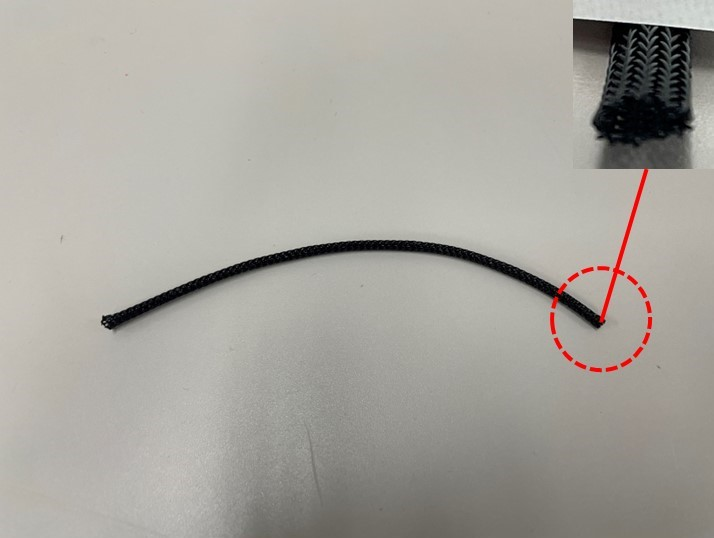
\includegraphics[scale=0.25]{image/messhu_hikaku_1.jpg}
    \subcaption{変化前}
    \label{fig:messhu_1}
  \end{minipage}
  %
  \begin{minipage}{0.49\hsize}
    \centering
    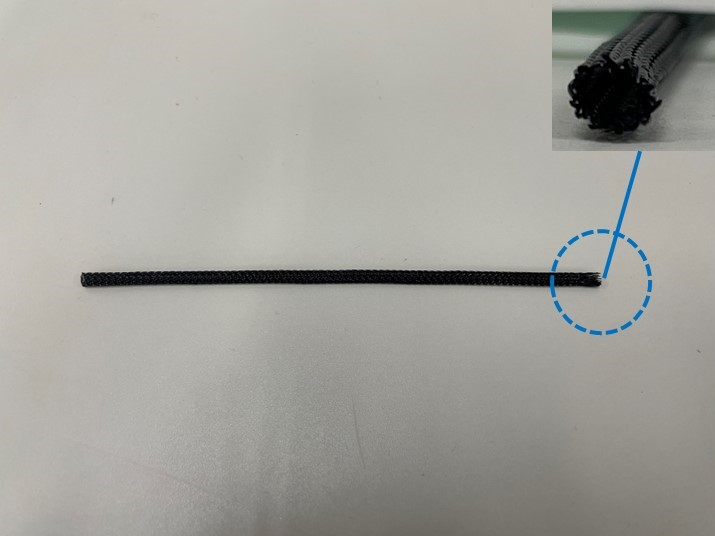
\includegraphics[scale=0.25]{image/messhu_hikaku_2.jpg}
    \subcaption{変化後}
    \label{fig:messhu_2}
  \end{minipage}
  %
  \caption{メッシュの熱可塑変化の様子}
  \label{fig:messhu_henka}
\end{figure}
%
\begin{figure}[!ht]
  %
  \begin{minipage}{0.49\hsize}
    \centering  
    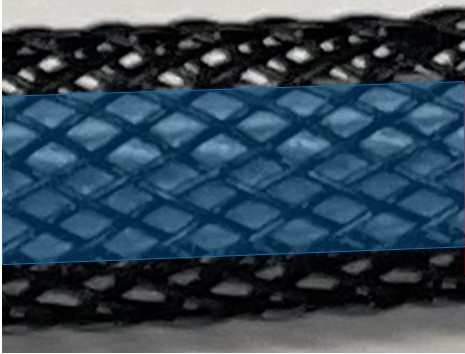
\includegraphics[scale=0.4]{image/hikaku_MPA_1.jpg}
    \subcaption{変化前}
    \label{fig:MPA_1}
  \end{minipage}
  %
  \begin{minipage}{0.49\hsize}
    \centering
    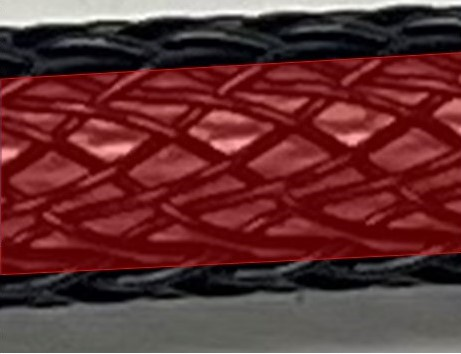
\includegraphics[scale=0.4]{image/hikaku_MPA_2.jpg}
    \subcaption{変化後}
    \label{fig:MPA_2}
  \end{minipage}
  %
  \caption{細径MPAの熱可塑変化の様子}
  \label{fig:MPA_henka}
\end{figure}
%
\begin{figure}[ht]
  \centering
  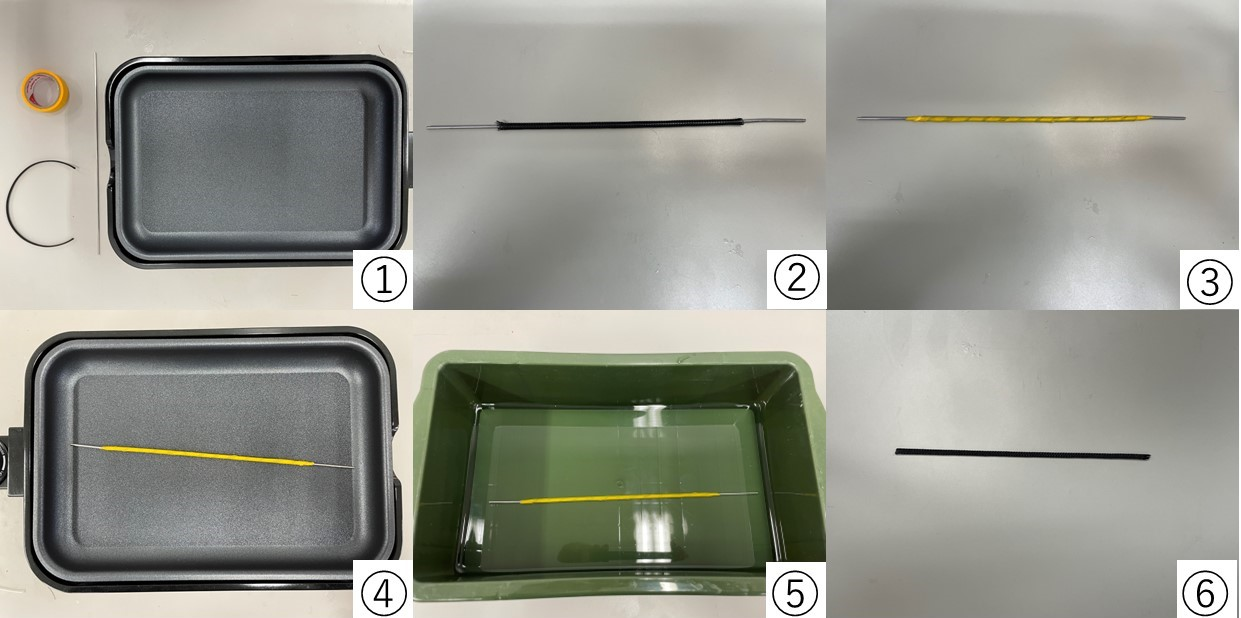
\includegraphics[scale=0.4]{image/messhu_tejyun.jpg}
  \caption{熱可塑変化の手順}
  \label{fig:messhu_method}
\end{figure}
%
%%%%%%%%%%%%%%%%%%%%%%%%%%%%%%%%%%%%%%%%%%%%%%%%%%%%%%%%%
\clearpage
\subsection{課題3:羽状角の変化に対する対応}
細径MPAを用いた羽状筋による腱の引き込みを模式図にしたものを図\ref{fig:ujyoukin_moshiki}に示す.
細径MPAが収縮することにより,腱が長手方向(赤い矢印の方向)へ引っ張られる.このとき,腱と細径MPAの成す角(羽状角)覇収縮前後で変化するため,細径MPAの腱および外殻への付着店は回転自由度を持つ必要がある.
しかし,先行研究\cite{hasegawa}で作製された細径MPAを用いた羽状筋では,では細径MPA端部の部品の角度が固定されていた.(図\ref{fig:ujyoukin_kako})
そのため,細径MPAが収縮した際に細径MPA自身が折れ曲がるように変形してしまい,腱を十分に引くことができず,関節可動域が狭くなる原因の1つとなっていた.
そこで本研究では細径MPAの端部に回転自由度を持たせる構造を考案した.図\ref{fig:tanbu_parts_new}に構造を示す.
図\ref{fig:tanbu_parts}\subref{fig:tanbu_parts}に示すように,MPA端部部品(部品\textcircled{\scriptsize 3})の軸部分を両側から挟むように,部品\textcircled{\scriptsize 1}\textcircled{\scriptsize 2}
を取り付ける部品\textcircled{\scriptsize 1}\textcircled{\scriptsize 2}にはMPA端部部品の軸と直行する向きに穴があけてある.組み立てたものを土台部品にとり付け,部品\textcircled{\scriptsize 1}\textcircled{\scriptsize 2}
を左右からネジで固定する(図c).このとき,ネジの先端が部品\textcircled{\scriptsize 1}\textcircled{\scriptsize 2}の穴部にはまることで,このネジが回転軸となり再帰依MPA端部が自由度を持つことができる.
また細径MPAの外殻側は圧縮空気を供給するために中空状になっており,そこへ$\phi$ 3mmのポリウレタンチューブを挿入したて接着剤で固定する.また土台部品も圧縮空気を供給するための流路が内部に設けてあり,
ポリウレタンチューブの他方そちらに挿入して接着剤で固定する.図19に実際に細径MPAを土台に組付けた様子を示す.
そこで本研究では細径MPAの収縮に応じて羽状角が変化する端部部品を開発した.開発した端部部品を図\ref{fig:tanbu_parts_new}\subref{fig:tanbu_parts}に示す.細径MPA端部の作製方法,手順を以下に示す.
%%%%%%%%%%%%%%%%%%%%%%%%%%%%%%%%%%%%%%%%%%%%%%%%%%%%%%%%%
%
\begin{figure}[ht]
  \centering
  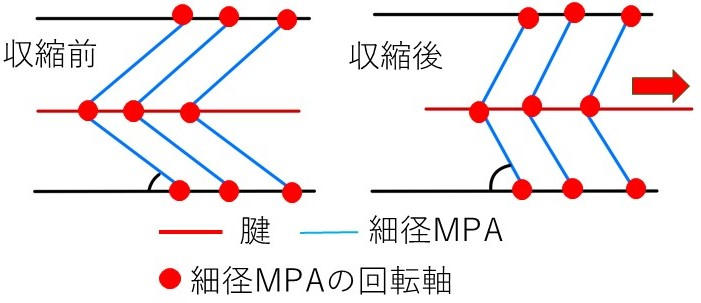
\includegraphics[scale=0.5]{image/ujyoukin.jpg}
  \caption{羽状筋の動作の模式図}
  \label{fig:ujyoukin_moshiki}
\end{figure}
%
\begin{figure}[ht]
  %
  \begin{minipage}{0.49\hsize}
    \centering  
    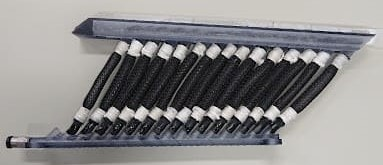
\includegraphics[scale=0.6]{image/yobi_syuseki.JPG}
    \subcaption{旧型羽状筋}
    \label{fig:ujyoukin_real_kako}
  \end{minipage}
  %
  \begin{minipage}{0.49\hsize}
    \centering
    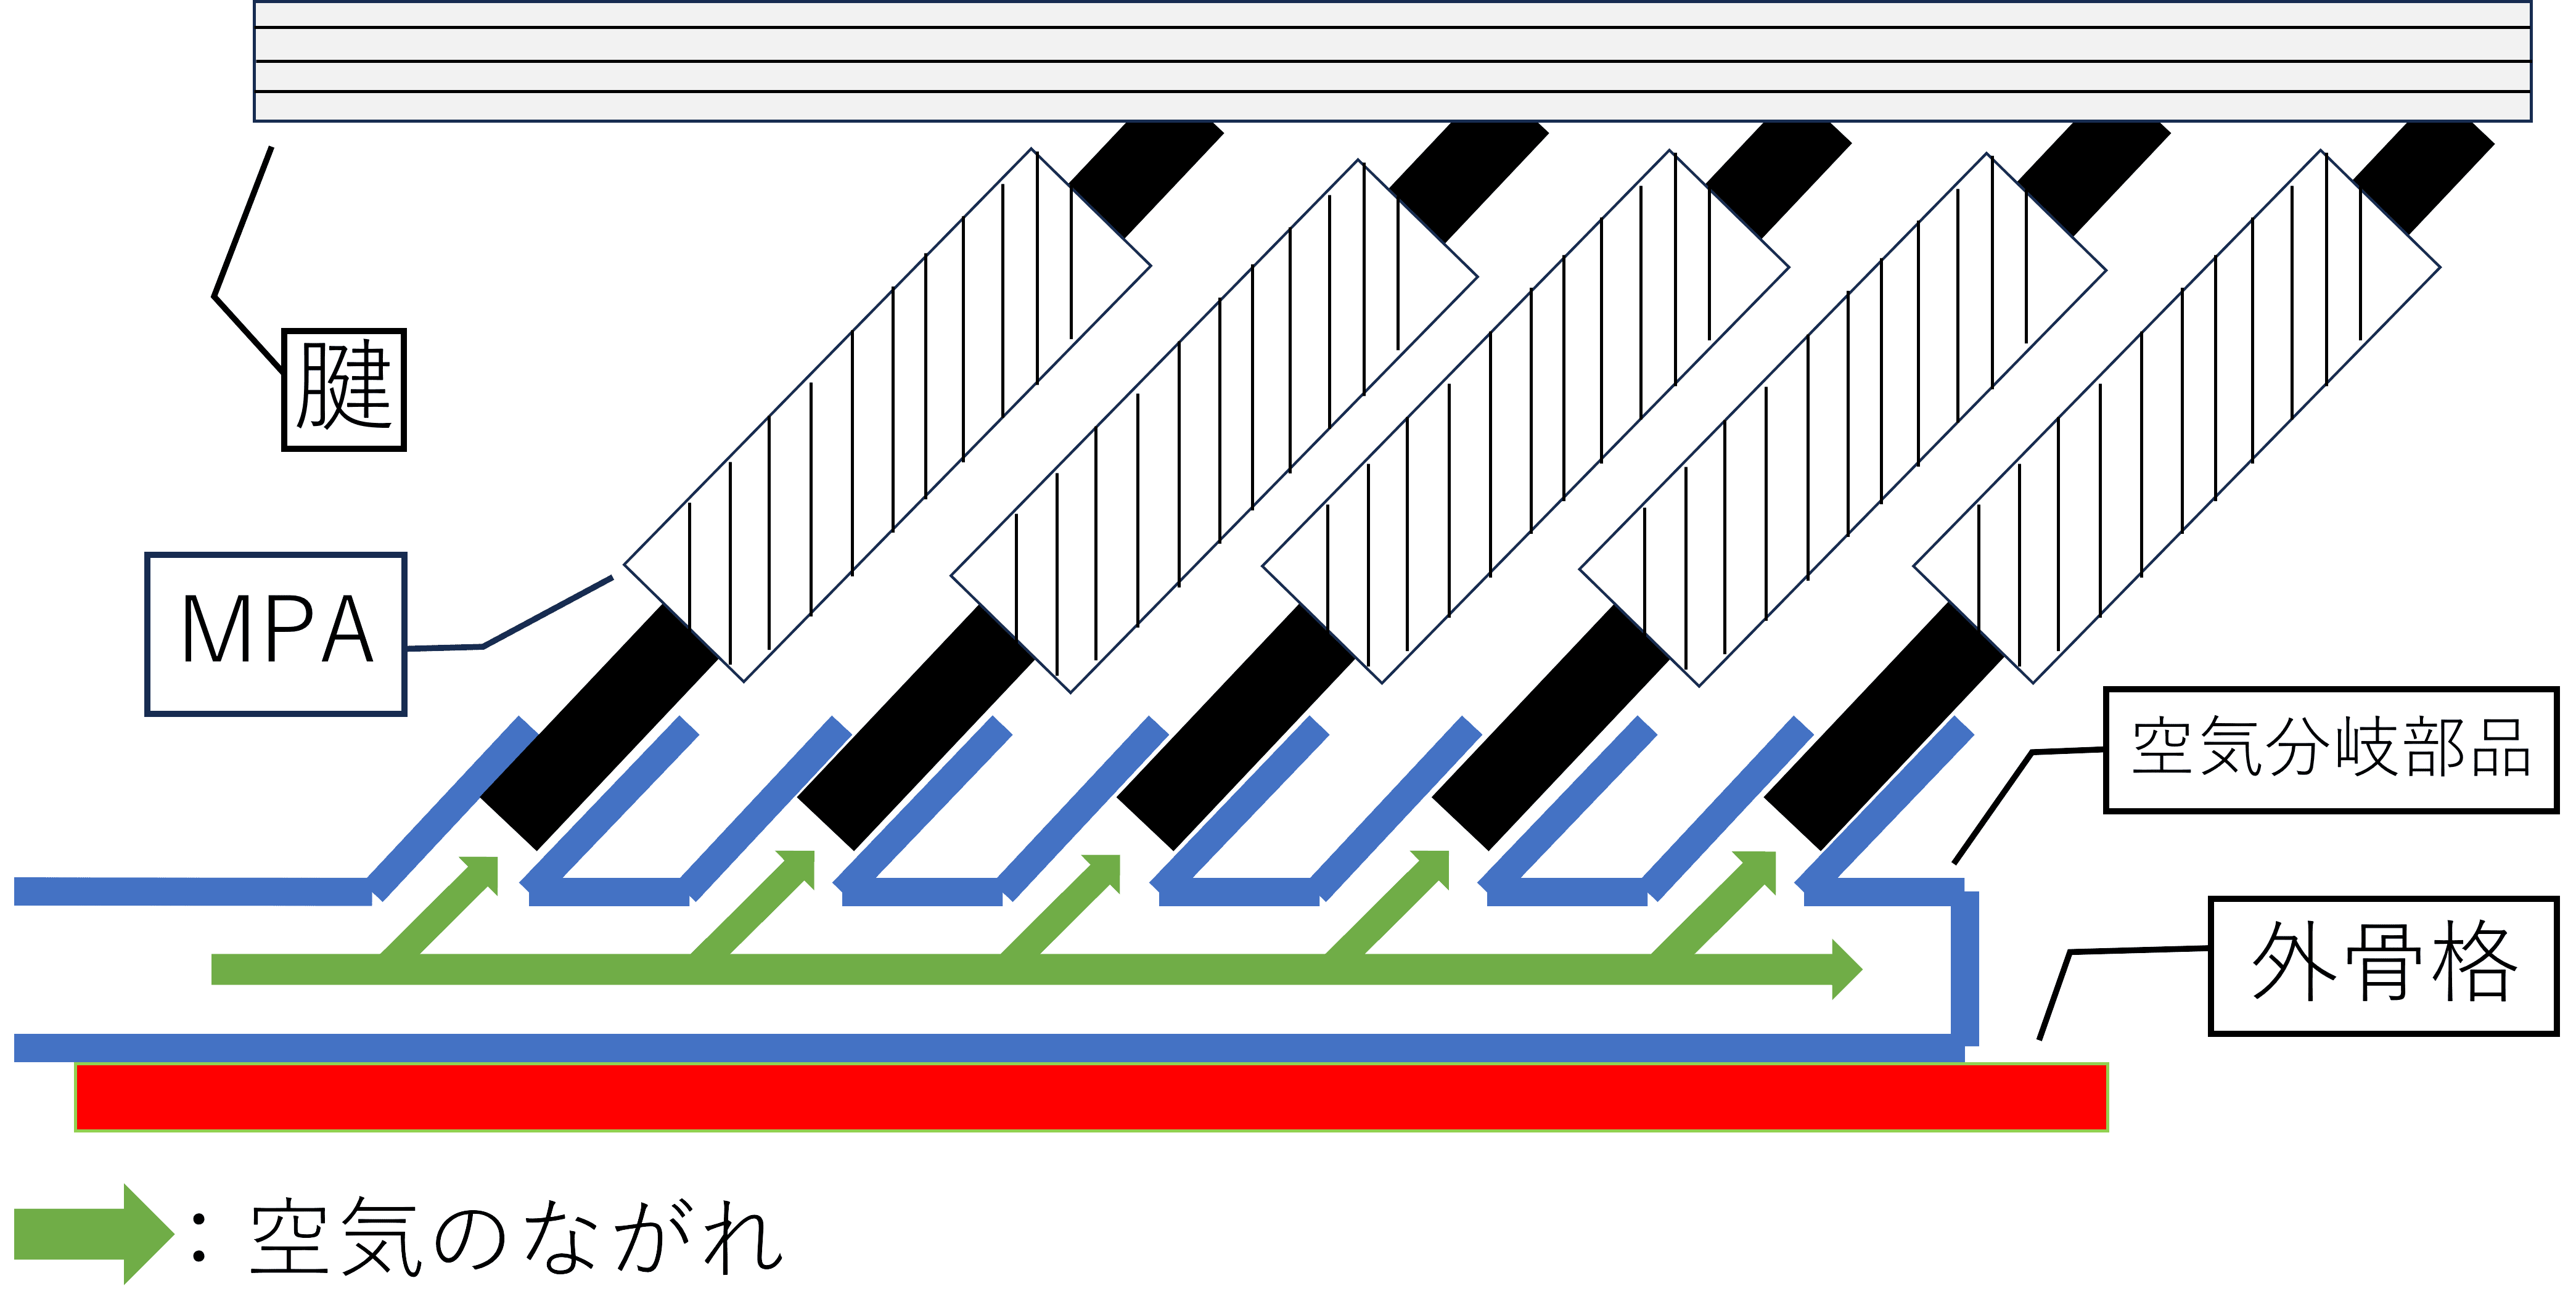
\includegraphics[scale=0.04]{image/air_moshiki.png}
    \subcaption{模式図}
    \label{fig:ujyoukin_moshiki_kako}
  \end{minipage}
  %
  \caption{先行研究で開発された羽状筋}
  \label{fig:ujyoukin_kako}
\end{figure}
%
\begin{figure}[ht]
  %
  \begin{minipage}{0.59\hsize}
    \centering  
    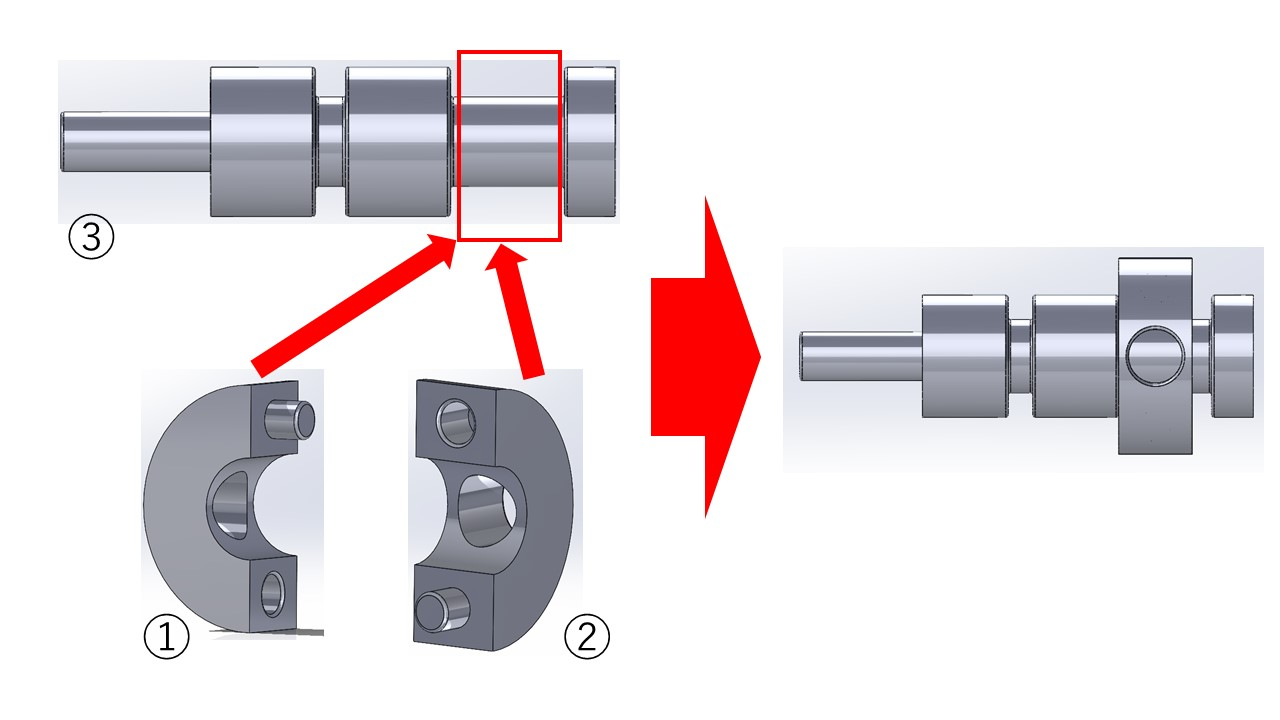
\includegraphics[scale=0.23]{image/tanbu_parts.jpg}
    \subcaption{組み立て方法}
    \label{fig:tanbu_parts}
  \end{minipage}
  %
  \begin{minipage}{0.39\hsize}
    \centering
    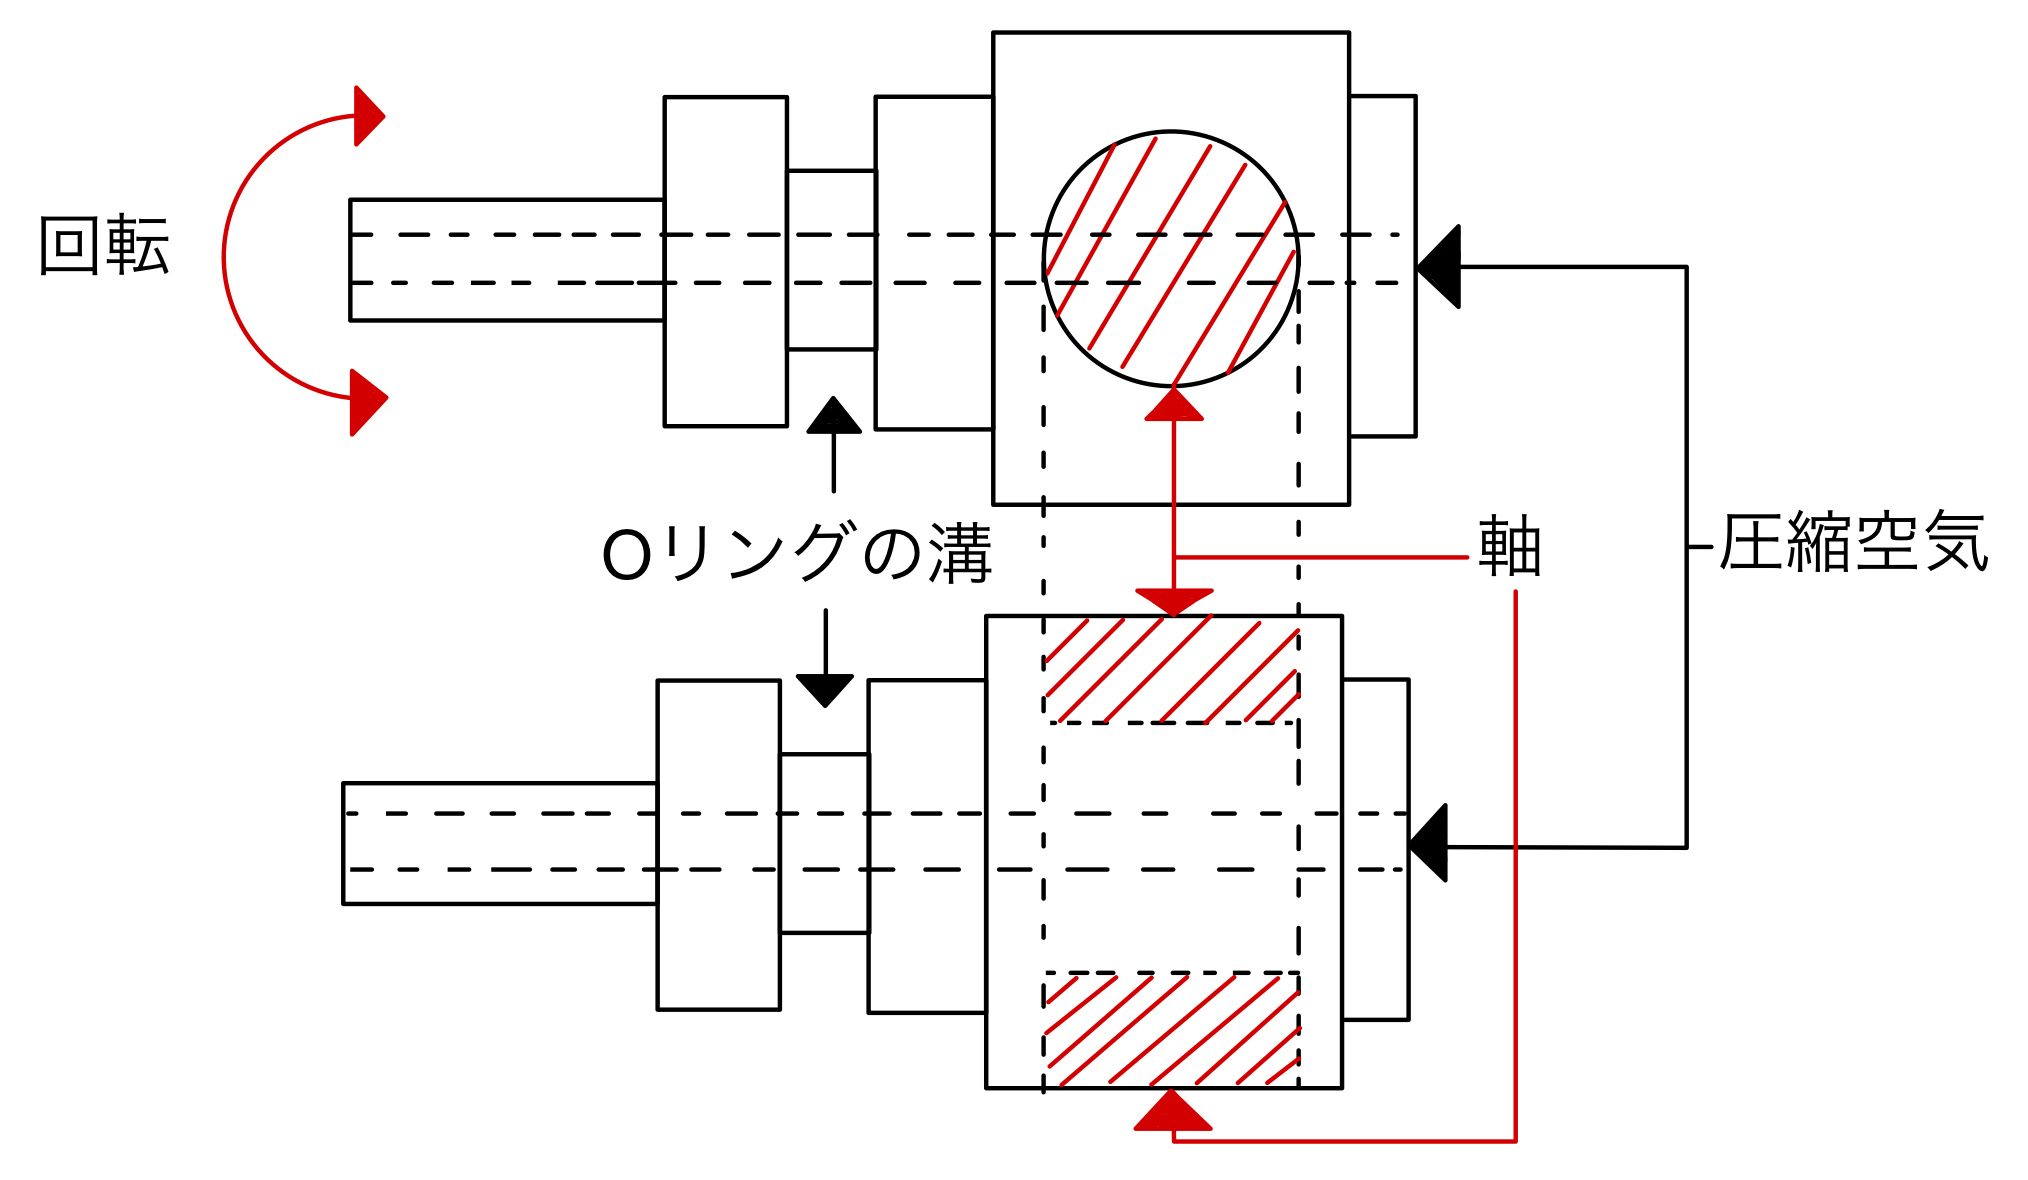
\includegraphics[scale=0.085]{image/MPA_irast.jpg}
    \subcaption{模式図}
    \label{fig:tanbu_moshikizu}
  \end{minipage}
  %
  \caption{先行研究で開発された羽状筋}
  \label{fig:tanbu_parts_new}
\end{figure}
%%%%%%%%%%%%%%%%%%%%%%%%%%%%%%%%%%%%%%%%%%%%%%%%%%%%%%%%%
\subsection{改良型細径羽状筋}
本研究で開発した改良型細径空圧羽状筋を図\ref{fig:ujyoukin_new}に示す.前述した先行研究の課題1,2,3の解決方法を取り入れて羽状筋を開発した.
図\ref{fig:ujyoukin_new}中の腱は柔軟な素材であるTPUを用いてFDM方式3Dプリンターで,細径MPA固定部品は光造形方式の3Dプリンターでそれぞれ作成した.
外骨格内部に配置可能な最大の長さの改良型細径空圧羽状筋を各節で作製した.その結果,解禁と平均で細径MPAの数が同じでそれぞれ1列ずつの構成となった.
長節では腱の上下ともに7本ずつ,腕節では腱の上側が5本で下側が4本,前節では腱の上下ともに4本ずつで羽状筋を作製した.
また,3章2節で述べた数理モデルのを用いた可動域の計算と作製の容易さから,細径MPAの長さは全て同じになるように作製した.
前述した先行研究の課題1,2,3の解決方法を取り入れて開発した改良型細径空圧羽状筋を図\ref{fig:ujyoukin_new}に示す.
\ref{fig:ujyoukin_new}中の腱は柔軟な素材であるTPUを用いてFDM方式3Dプリンターで,外殻部分はPLAを用いてFDM方式の3Dプリンターで,細径MPA固定部品覇光造形方式の3Dプリンターでそれぞれ作成した.
3.2で述べたように,羽状角を 20度かつすべての細径MPAの長さは等しいという条件のもと,可能な限り外骨格内部に細径MPAを配置した.
また外殻の幅の制約から,すべての節で屈筋伸筋は一列ずつとした.長節においては屈筋伸筋ともに上下に7本ずつ,7対14筋能状筋とした.
同様に前節は4対8筋とした.腕節では屈筋伸筋ともに腱の上側が5本,下側が4本の非対称な羽状筋とした.
これは可能な限り空間内に多数の細径MPAを配置し,腱を引き込む力を大きくするためである.
%%%%%%%%%%%%%%%%%%%%%%%%%%%%%%%%%%%%%%%%%%%%%%%%%%%%%%%%%
%
\begin{figure}[!hb]
  \centering
  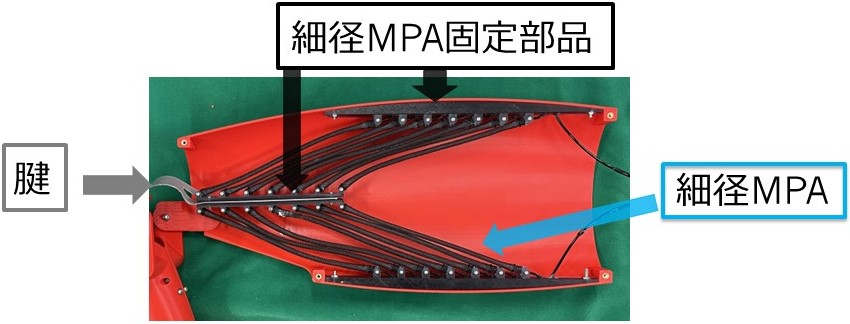
\includegraphics[scale=0.53]{image/uyjoukin_new.jpg}
  \caption{改良型細径空圧羽状筋}
  \label{fig:ujyoukin_new}
\end{figure}
%
%%%%%%%%%%%%%%%%%%%%%%%%%%%%%%%%%%%%%%%%%%%%%%%%%%%%%%%%%
%本研究で用いる3 mmの細径MPAの作製方法について説明する.
%構造は2.1節で述べた従来のMPAと同様,シリコンゴムチューブをナイロン繊維メッシュで覆ったシンプルなもので,0.4~0.6 MPaで駆動し収縮率は約20 %である.
%おおまかな作製手順を図\ref{fig:shingata_sakuseihouhou}に示す.
%端部の締結方法はOリングを用いる方法を採用した.
%図中\textcircled{\scriptsize 1}に示した物品が作製に必要なもので左から以下の通りである.
%
%\begin{itemize}
%  \item PPX(瞬間接着剤) メーカー:セメダイン 品番:CA-522
%  \item シリコンゴムチューブ 2×3(内径×外径) メーカー:タイガースポリマー 品番:SR1554
%  \item ポリウレタンチューブ 2×1.2(外径×内径) メーカー:PISCO 品番:UB0212-20-B
% \item 編組チューブ 1×5(最小径×最大径) メーカー:モノタロウ 品番:-
%  \item 光造形で作製した細径MPA端部部品
%\end{itemize}
%
%以下,作成手順である.
%
%\begin{enumerate}
%  \item まず初めにシリコンゴムチューブを任意の長さで切り,ナイロンメッシュをシリコンゴムチューブより5 cm程長く切る
%  \item シリコンゴムチューブの両端をそれぞれ光造形の部品の溝に差し込み,部品とシリコンゴムチューブの間に接着剤を塗布する(図中\textcircled{\scriptsize 2})
%  \item 接着剤が十分に乾いたら編組チューブを被せる(図中\textcircled{\scriptsize 3})
%  \item ナイロンメッシュを押さえつけ,かつ光造形のOリング固定溝にはまるようにOリングを配置する.固定する際にナイロンメッシュが緩まないようにOリングを固定する(図中\textcircled{\scriptsize 4})
%  \item 締結した部分に接着剤を塗布し,緩まないようにする
%  \item 接着剤が十分に乾いたら余分なナイロンメッシュを切り取る(図中\textcircled{\scriptsize 5})
%  \item ポリウレタンチューブを光造形の部品に差し込み,部品とポリウレタンチューブの間に接着剤を塗布し乾燥させて完成
%\end{enumerate}
%%%%%%%%%%%%%%%%%%%%%%%%%%%%%%%%%%%%%%%%%%%%%%%%%%%%%%%%%
%\begin{figure}
%  \centering
%  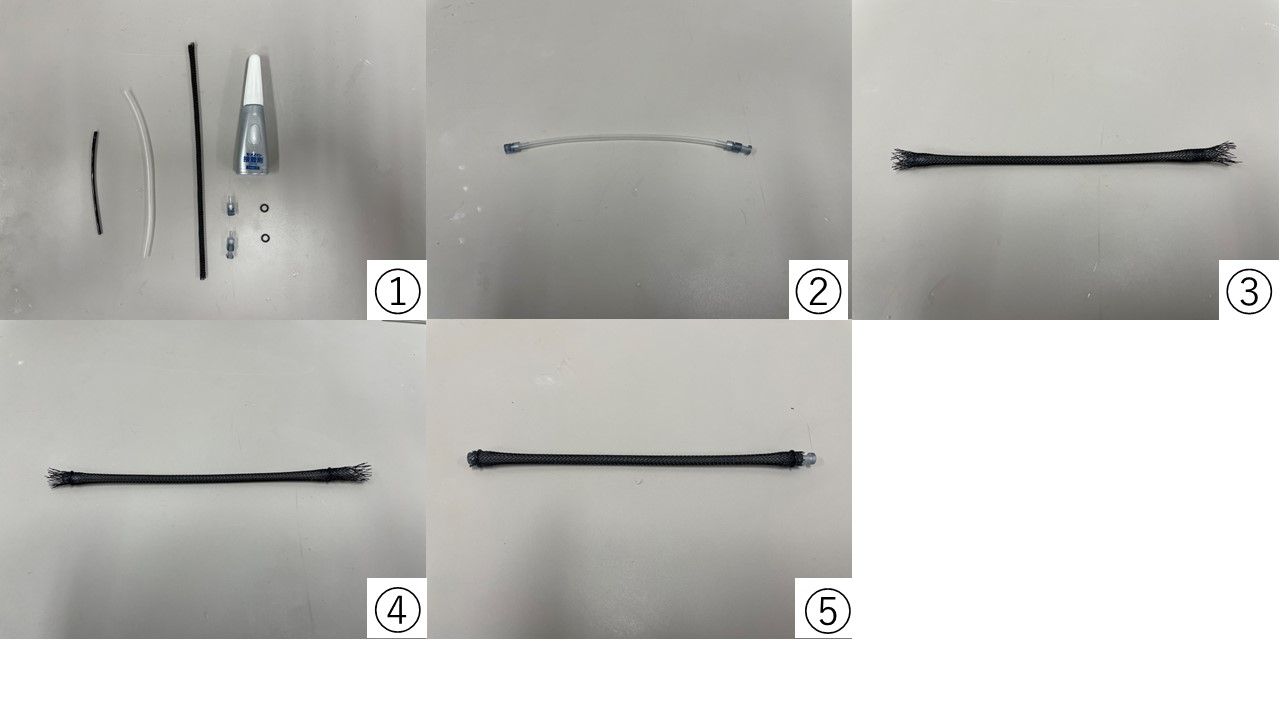
\includegraphics[scale=0.4]{image/sakusei.jpg}
%  \caption{改良型細径MPAの作製方法}
% \label{fig:shingata_sakuseihouhou}
%\end{figure}
%%%%%%%%%%%%%%%%%%%%%%%%%%%%%%%%%%%%%%%%%%%%%%%%%%%%%%%%%


% 必要に応じて章を増やす,またファイル名もsec2, sec3である必要はない
% このmain.texが置いてあるディレクトリ内にある「chapters」フォルダ以下に
% 自分がわかりやすい名前のtexファイルを作成し,\include{chapters/*****}で
% 呼び出せば良い
%\newpage
\section{結言}
      % 結言
%\newpage
\Section{謝辞}
本研究を進めるにあたり,数多くの助言や提案,資料の添削など最後まで手厚くサポー
トしていただいた中西大輔先生に心より感謝いたします.また,苦しい時間や楽しい時間
をともにした研究室の皆様に厚くお礼申し上げます. % 謝辞
% できればbibtexを使ってください
\newpage
\Section{参考文献}

\bibliographystyle{junsrt}
\bibliography{reference.bib}
% \begin{thebibliography}{9}
% \end{thebibliography}


    % 参考文献

\end{document}
